\documentclass[12pt, a4paper]{article}
\usepackage{epigraph}
\usepackage[dutch]{babel}
\usepackage{apacite}
\usepackage[normalem]{ulem}
\usepackage{xcolor}
\usepackage{enumerate}
\usepackage{graphicx}
\usepackage{caption}
\graphicspath{ {./images/} }
\captionsetup{font=small}

\setlength\epigraphwidth{10cm}
\setlength\epigraphrule{0pt}

\title{Normaliseren met SlimStampen \\ \large Over de mogelijke waarde van een digitaal leermiddel als onderdeel van de montessorimethode} 
\author{Marijn van der Meer\\ Leergang Montessori Meesterschap \\ Metis Montessori Lyceum Amsterdam}

\date{Voorjaar 2024}

\begin{document}
\maketitle
\thispagestyle{empty}
\pagebreak
\thispagestyle{empty}
\tableofcontents
\pagebreak
\thispagestyle{empty}
\epigraph{“The child whose attention has once been held by a chosen object, while he concentrates his whole self on the repetition of the exercise, is a delivered soul in the sense of the spiritual safety of which we speak. From this moment there is no need to worry about him - except to prepare an environment which satisfies his needs, and to remove obstacles which may bar his way to perfection.”}{--- \textup{Dr. Maria Montessori}\\ The Absorbent Mind, p. 247}
\pagebreak

\section*{Voorwoord}

Voor u ligt het praktijkonderzoeksverslag \emph{Normaliseren met SlimStampen}, geschreven in het kader van de afstudeereisen van de leergang Montessori Meesterschap.

Het schrijven van dit onderzoeksverslag was voor mij een goede aanleiding om mijn lang gekoesterde wens tot het leren van de opmaaktaal \LaTeX  te vervullen. Dit heeft het starten met schrijven iets vertraagd, maar het is goed en leuk om weer eens iets heel nieuws te leren. Goed om te ervaren wat leerlingen ervaren en leuk omdat ik iemand ben die van leren houdt en het leren op zichzelf leuk vind.

Het onderwerp van mijn onderzoek: de waarde van het SlimStampen algoritme in het montessorionderwijs, ligt mij aan het hart. Ik was hier al mee aan de slag en ik ga ermee door. Door dit onderzoek vergroot ik mijn deskundigheid in de waarde van dit algoritme voor het montessorionderwijs.

Ik ben dank verschuldigd aan Hedderik van Rijn, hoogleraar cognitieve wetenschappen en neurowetenschappen aan de Rijksuniversiteit Groningen, voor de jarenlange vriendschap en de fijne vakanties op onder andere Terschelling om al wandelend of 's avonds bij het eten te praten over de mogelijkheden van het SlimStampen algoritme dat hij met zijn vakgroep ontwikkeld heeft. Daarmee ook dank aan Maarten van der Velde van SlimStampen/MemoryLab en Gesa van den Broek van de Universiteit Utrecht voor hun enthousiasme voor mijn onderzoek, het meedenken over de vragenlijst en voor de fijne en duurzame samenwerking die wij hebben.

Marcelle Peeters dank ik voor het meelezen en mij groot brengen tot een leergierige en enthousiaste docent. Amber Beckers, Noah en Zoë voor hun geduld en steun bij mijn gesprekken aan tafel en overal tussendoor. Jeroen Dercksen voor het ontwerp van het omslag. Mijn Metis collega's en de leerlingen voor hun collegialiteit, toewijding en dagelijkse doses gezelligheid. Zoals Maria Montessori schreef: ''To serve the children is to feel one is serving the spirit of man, a spirit which has to free itself. The difference of level has truly been set not by the teacher but by the child. It is the teacher who feels she has been lifted to a height she never knew before. The child has made her grow till she is brought within his sphere.'' \cite[p.257]{Montessori2016}\\

En tenslotte dank ik de MSA voor het creëren van deze opleiding en mijn studiebegeleiders voor hun feedback en inspirerende lessen.
Ik hoop dat dit onderzoek een bijdrage zal leveren aan beter onderwijs en wens u veel leesplezier.\\

--- \textup{Marijn van der Meer, Amsterdam, mei 2024.}

\pagebreak
\begin{abstract}
    Het doel van dit onderzoek was om, op grond van een literatuurstudie en een enquête onder leerlingen, inzicht te krijgen in de waarde van SlimStampen op een middelbare montessorischool. Ik heb de waarde vertaald naar een viertal belangrijke kenmerken van het montessorionderwijs: de voorbereide omgeving, normalisatie, motivatie en leerstrategieën. Daarnaast heb ik het gebruik van SlimStampen geëvalueerd door middel van een enquête onder de leerlingen.
    
    Uit de data uit de enquête blijkt dat leerlingen positief zijn over SlimStampen als montessorimateriaal. Het zelf indelen van de tijd, de helderheid van het materiaal en het vervangen van toetsen door SlimStampen wordt zeer gewaardeerd. Ikzelf zie SlimStampen ook als leermiddel voor het aanleren van leerstrategieën, zoals herhalen en ophalen, dit blijkt zowel uit de theoretische vergelijking als uit de enquête. Veel leerlingen zijn al bekend met deze leerstrategieën. Leerlingen geven aan zich goed te kunnen concentreren tijdens het gebruik van SlimStampen. Zij laten zich niet snel afleiden als ze met deze taak bezig zijn. Het werken met SlimStampen geeft de leerlingen meer gevoel van autonomie.
    
    SlimStampen helpt bij de motivatie voor leerlingen. Ze leren rijtjes woorden liever met SlimStampen dan op een andere manier. Het leren met SlimStampen geeft een positief gevoel achteraf. De leerlingen vinden het fijn om meer hun eigen tijd in te kunnen delen. Ze voelen zich zekerder over hun kunnen op school door SlimStampen en hebben het idee dat ze nu hogere cijfers halen. Kortom SlimStampen zorgt bij veel leerlingen voor een gevoel van competentie.

    De conclusie is dat SlimStampen van waarde is voor het montessorionderwijs. Het past binnen de kenmerken van het montessorionderwijs en draagt bij een stimulerende voorbereide omgeving, aan normalisatie, de motivatie en gebruikt effectieve leerstrategieën van de leerlingen. Het onderzoek wordt afgesloten met een aantal aanbevelingen voor het vervolg.
\end{abstract}
\newpage
\section{Aanleiding en probleemstelling}
In september 2022 ben ik vol enthousiasme aan de leergang Montessori Meesterschap begonnen. Ik stond op dat moment vijf jaar voor de klas op een Montessorischool. Ik voelde me als een vis in het water, dit onderwijs begreep ik, maar ik kon moeilijk uitleggen waarom. 
Ik vond het daarom dat het tijd was om uit te zoeken waarom het montessorionderwijs zo bij mij past en ik zo veel geloof had in het concept montessorionderwijs. 

Het Metis Montessori Lyceum is onderdeel van de Montessori Scholengemeenschap Amsterdam. Een schoolorganisatie waaronder zes middelbare scholen in Amsterdam vallen met allemaal een montessori-signatuur.
Het is een open, jonge en innovatieve school. De positieve uitstraling van de school wordt voor een groot deel bepaald door de profielen die de leerlingen bij aanvang kiezen en door de docenten die aan deze profielen verbonden zijn. Daarbij speelt mee dat het een relatief jonge school is, met een jong team van enthousiaste en leergierige docenten. Voor de profielvakken bestaan geen methoden die de docenten kunnen aanschaffen en volgen. Dit vergt van de docenten een continue ontwikkeling en verbetering van het materiaal. De onderwijskundige principes van Maria Montessori zijn daarbij richtgevend. Individueel en als team lukt het steeds beter deze principes te vertalen in concrete handelingen voor dit middelbare onderwijs.

Als zij-instromer voel ik mij als een jonge docent: elke dag valt er veel te leren en bijna elke dag gebeurt er iets dat ik nog niet eerder heb ervaren. Ik ben iemand die graag wil leren van collega’s en met collega’s, van leerlingen en met leerlingen. Ik voel mij  op deze school enorm op mijn plek. In deze context heb ik een aantal jaren geleden SlimStampen geïntroduceerd. Eerst door zelf kleine experimenten met leerlingen te doen. Vervolgens door hierover te vertellen en het voor te doen. Leerlingen en collega’s werden langzaam maar zeker enthousiast. Zo leerde ik de (on)mogelijkheden van implementatie en toepassing steeds beter kennen.

SlimStampen is een adaptief leeralgoritme dat het leren van feitenkennis sneller en makkelijker maakt. Het algoritme maakt van iedere gebruiker een model van het geheugen en gebruikt dit om voor iedereen het optimale leerproces te bepalen. Doordat het systeem voor elke leerling het leerproces registreert kan het algoritme feedback geven aan de leerling en de docent over het leerproces en heel nauwkeuring inschatten of de feiten worden beheerst. Daarmee kan het SlimStampen algoritme bepaalde toetsen vervangen of aanvullen. Zo kunnen we van summatief toetsen naar summatief leren gaan. Ik heb hier vorig jaar uitgebreid over geschreven en verwijs voor verdere informatie naar \emph{SlimStampen met Maria} \cite[]{Marijn23} of de uitleg die te vinden is op www.memorylab.nl/wetenschap.

SlimStampen is ontwikkeld door de vakgroep van Hedderik van Rijn aan de Universiteit van Groningen en is sinds 2023 ondergebracht bij de start-up MemoryLab. Hier wordt het algoritme en de toepassing continu geëvalueerd en doorontwikkeld op basis van nieuwe theoretische inzichten en de ervaringen in de praktijk. Samen met de Universiteit Utrecht heeft de Montessori Scholengemeenschap Amsterdam (MSA) subsidie gekregen van het Nationaal OnderwijsLab AI (NOLAI) om samen met MemoryLab een driejarig onderzoek te doen naar het vervangen van een toets door een leeralgoritme. Een vereiste voor de subsidie was dat de onderzoeksvraag uit de praktijk moest komen. Ik heb de subsidie aangevraagd en ben nu de coördinator van dit project namens de MSA.

Vorig jaar schreef ik mijn montessori-interventie over het invoeren van SlimStampen op een montessorischool. \cite[]{Marijn23} Door deze praktische en theoretische verdieping heb ik ervaring en kennis opgedaan over montessorimaterialen, over SlimStampen en over het overtuigen en meenemen van collega's en leerlingen bij het invoeren van een leeralgoritme. Tegelijkertijd resulteerde dit onderzoek in nieuwe vragen. Dit afstudeeronderzoek is voor mij een uitgelezen gelegenheid om met die vragen aan de slag te gaan. Concluderend kom de volgende probleemstelling naar voren: Wat is de waarde van SlimStampen op een middelbare montessorischool?\\

Dit praktijkonderzoek start met de probleemverkenning in hoofdstuk 2. Vervolgens beschrijf ik in hoofdstuk 3 de doelstelling van dit onderzoek, inclusief de onderzoeksaanpak. In hoofdstuk 4 volgt het theoretisch kader, met aansluitend in hoofdstuk 5 de conclusies van het literatuuronderzoek. In hoofdstuk 6 beschrijf ik de onderzoeksresultaten om tenslotte, in hoofdstuk 7, af te sluiten met conclusies en aanbevelingen.
\newpage
\section{Probleemverkenning}
Vorig jaar heb ik voor het Montessori Meesterschap een interventie beschreven over SlimStampen en daarbij de theoretische relatie tussen SlimStampen en de onderwijsprincipes van Maria Montessori gelegd \cite[]{Marijn23}. De conclusie was dat SlimStampen een effectieve leermethode is, die theoretisch past binnen het montessorionderwijs.
De positieve resultaten van de onverwachte toets die ik gaf binnen mijn experiment met het leren van topografie met behulp van SlimStampen vormden het begin van het breder invoeren van dit leeralgoritme op het Metis Montessori Lyceum. Niet alleen bij mijn lessen en niet alleen bij het vak aardrijkskunde, maar ook bij andere lessen, door andere docenten, bij andere vakken. 
Inmiddels is SlimStampen bij een aantal vakken een vast onderdeel geworden van het curriculum. Dit is sneller gegaan dan ik had durven hopen. Alle leerlingen van het Metis hebben in meer of mindere mate ervaring met het gebruik van SlimStampen. De meeste leerlingen en docenten zijn enthousiast, maar dat geldt niet voor iedereen. In een voortgangsgesprek met mijn leidinggevende kwamen we samen tot de conclusie dat het goed zou zijn om nader onderzoek te doen naar het gebruik van SlimStampen. Dat zou ons een basis geven om het gesprek met docenten en leerlingen meer evidence-based te kunnen voeren en ook om zelf deze interventie nog beter te leren doorgronden. Zowel mijn leidinggevende als ikzelf zien SlimStampen als een kans om het onderwijs te verbeteren. Het probleem is dat wij vooralsnog de nodige kennis missen om alle docenten hierin mee te nemen.

De essentie van het leeralgoritme wordt op basis van de nieuwste wetenschappelijk inzichten continu geëvalueerd en bijgesteld door MemoryLab. Dit alles is volledig toegankelijk gemaakt op hun website (www.memorylab.nl
/wetenschap). Door het gezamenlijke driejarige onderzoek van de MSA, MemoryLab en de Universiteit Utrecht, dat dankzij de subsidie van NOLAI mogelijk is, zijn wij goed aangehaakt bij deze ontwikkelingen. Het is dus zaak om dit onderzoek toe te spitsen op kennis over de toepassing van SlimStampen in onze specifieke situatie: het Metis Montessori Lyceum. De docenten ontwikkelen al hun onderwijs binnen de principes van montessorionderwijs. Het is belangrijk om te weten of en hoe SlimStampen bijdraagt aan de kenmerken van ons onderwijs. Een andere belangrijke vraag voor de verdere implementatie van SlimStampen is de vraag hoe de leerlingen oordelen over het gebruik van SlimStampen. Waarom gebruiken leerlingen het wel of niet? En als ze het gebruiken zijn ze er dan tevreden over? De motivatie van de leerling is voor docenten een belangrijk punt.
\newpage
\section{Doelstellingen}
Het doel van dit onderzoek is om, op grond van een literatuurstudie en een enquête onder leerlingen, inzicht te geven in de waarde van SlimStampen in een middelbare montessorischool. Dit hoofddoel wordt beantwoord aan de hand van twee deelvragen:
\begin{itemize}
    \item Welke kenmerken van het montessorionderwijs zijn aan de orde bij het gebruik van SlimStampen?
    \item Hoe beoordelen de leerlingen van het Metis Montessori Lyceum het gebruik van SlimStampen?
\end{itemize}

\subsection{Beschrijvend onderzoek}
Voor het beantwoorden van deelvraag 1 leg ik, door middel van literatuuronderzoek, de relatie tussen kenmerken van het montessorionderwijs en SlimStampen. Ik behandel daarbij de volgende kenmerken: 
\begin{enumerate}
    \item Voorbereide omgeving
    \item Normalisatie
    \item Motivatie
    \item Leerstrategieën (herhaling van de oefening)
\end{enumerate}
Ik heb gekozen voor deze kenmerken omdat ik door mijn ervaring met SlimStampen en montessorionderwijs het idee heb dat deze kenmerken in SlimStampen zitten. Door gesprekken met collega's, vrienden, leerlingen en wetenschappers heb ik dit idee getoetst. Nu wil ik deze aanname verdiepen door middel van literatuuronderzoek en toetsen of dit door leerlingen ook zo ervaren wordt. 

\subsection{Evaluerend onderzoek}
Ik kan uiteraard niet direct vragen aan leerlingen of zij zich bijvoorbeeld  ''beter genormaliseerd'' voelen door het gebruik van SlimStampen, dus daar moet ik indicatoren voor gaan bedenken. Ook zal ik eerst vast moeten stellen wat Montessori heeft beschreven over de voorbereide omgeving, de normalisatie, motivatie en leerstrategieën.

In het evaluerend onderzoek leg ik de leerlingen een vragenlijst voor.
De vragenlijst is samengesteld op basis van de uitkomsten van het literatuuronderzoek, vragen over het oordeel van leerlingen over SlimStampen en gesprekken met mijn studiebegeleiders, collega's en wetenschappers. 
Zo krijg ik kennis over de vraag of die aansluiting van SlimStampen bij de kenmerken in de praktijk, door de leerlingen wordt bevestigd en daarbij antwoord op deelvraag 2: kennis over het oordeel van leerlingen over SlimStampen. 

Met deze opgedane kennis kan ik in de toekomst in gesprek gaan met betrokken collega's binnen de MSA, over of en hoe SlimStampen breder ingezet kan worden op onze scholen.

\newpage
\section{Theoretisch kader}
Mijn theoretisch kader is gebaseerd op twee invalshoeken: de theorie van het montessorionderwijs en de theorie achter het leeralgoritme SlimStampen. Op basis van mijn onderzoeksvraag beschrijf ik bij elk kenmerk (zie 3.1) eerst de montessoritheorie en eventuele andere onderwijstheorieën die hiervoor relevant zijn. In de conclusie van deze literatuurstudie zal ik de montessoritheorie verbinden met SlimStampen en conclusies trekken. 
Maria Montessori hechtte veel waarde aan wetenschappelijk onderzoek en was van mening dat hervormingen in het onderwijs gebaseerd moesten zijn op (nieuwe) wetenschappelijke inzichten. \cite[p.351]{Lillard}.
Ook voor SlimStampen is een wetenschappelijk fundament essentieel. Het algoritme van SlimStampen is gebaseerd op inzichten uit de cognitieve psychologie \cite[]{Rijn09}.

\subsection{Voorbereide omgeving}
De omgeving en in het bijzonder de schoolomgeving is cruciaal voor de ontwikkeling van het kind. \cite[p.212-217]{Montessori2012}.
''Men moet een omgeving scheppen, waarin het kind de groeiende behoefte van zijn leven kan bevredigen. In deze omgeving moet hij derhalve ook het voedsel vinden, waarmede hij zijn kennis kan verrijken en zijn verstandelijke vermogens kan ontwikkelen'' \cite[p.93]{Montessori1952}. 

De schoolomgeving zorgt dus voor een mentale ontwikkeling van het kind. Volgens Montessori kent de mentale ontwikkeling drie belangrijke aspecten: vrije keuze in werk, herhaling van de oefening en concentratie. \cite[p.202]{Montessori2020}
De docent maakt deel uit van de voorbereide omgeving. Het kind, de docent en de omgeving vormen een drie-eenheid.

Een montessoriomgeving zorgt volgens Lillard om drie redenen voor concentratie. Als eerste de voorbereide omgeving, met het daarbij behorende aantrekkelijke materiaal. Als tweede een werkcyclus van drie uur en als laatste zo min mogelijk afleiding die concentratie zou kunnen verstoren. \cite[p.122-123]{Lillard}. Over de vereisten van educatief montessorimateriaal heb ik vorig jaar uitgebreid geschreven in mijn interventie. Het materiaal heeft een vijftal kenmerken. De eerste is de ''controle van de fout'', de tweede ''de isolatie van de eigenschap'', de derde ''het materiaal is esthetisch'', de vierde ''het materiaal roept de aandacht en interesse van het kind op'' en het laatste kenmerk is ''de beperkte hoeveelheid'' (zie \cite[]{Marijn23}, \cite[]{Montessori2017}). Ik kwam vorig jaar tot de conclusie dat SlimStampen vier van de vijf kenmerken van montessorimateriaal in zich heeft. Alleen de beperkte hoeveelheid is met een online tool uiteraard niet aanwezig. De werkcyclus van drie uur is op het voortgezet onderwijs meestal niet haalbaar. De hoeveelheid vakken en de bijbehorende lokaalwisselingen maken dit niet mogelijk, maar is de diepere concentratie die Montessori beschrijft met SlimStampen wel mogelijk? Daar kom ik later in paragrafen 4.3 en 4.5 nog op terug.
Mario Montessori beschrijft in zijn boek dat het materiaal ook ''vormend'' moet zijn. Het moet helpen bij het vormen van de persoonlijkheid. Hij geeft aan dat dit voornamelijk gebeurt door een ''beperkte hoeveelheid'' van het materiaal in de klas te hebben, hierdoor moeten leerlingen leren dat ze soms moeten wachten en dat niet alles altijd maar beschikbaar is \cite[p.88]{Mario}. Materialen kunnen ook op andere manieren vormend zijn. Daar kom ik in paragraaf 4.5 op terug.

\subsection{Normalisatie}
Binnen het montessorionderwijs heeft de term ''normalisatie'' een bijzondere betekenis. Het gaat er niet om leerlingen ''normaal'' te laten worden, in de term van gemiddeld of gewoon. Ook betekent het niet dat leerlingen geforceerd moeten worden zich te gedragen en ''normaal'' gedrag opgelegd moet worden. Maria Montessori gebruikt de term ''normalisatie'' voornamelijk voor een bepaalde ontwikkeling van het kind die zij heeft waargenomen en die zij bijvoorbeeld uitvoerig beschrijft in \emph{The Absorbent Mind} en \emph{The 1946 London Lectures}.
Voor Montessori is begrip ''normalisatie'' heel breed. Er bestaat voor Maria Montessori een genormaliseerd gedrag op school. Dit gedrag op school zal leiden naar de ontwikkeling die Maria Montessori voor ogen heeft, maar is voor in het onderwijs veel praktischer van aard. Hier kan het onderwijs direct iets mee:
''Normalization comes about through ''concentration'' on a piece of work. For this we must provide 'motives for activity' so well adapted to the child’s interests that they provoke his deep attention. Their success in this is dependent on the use of the objects for the purposes they are designed to serve, a thing, which is also conducive to the child’s 'mental order.' […] 
Only ''normalized'' children, aided by their environment, show in their subsequent development those wonderful powers that we describe: spontaneous discipline, continuous and happy work, social sentiments of help and sympathy for others. […] An interesting 
piece of work, freely chosen, which has the virtue of inducing concentration rather than fatigue, adds to the child’s energies and mental capacities, and leads him to self-mastery'' \cite[pp. 185-186]{Montessori2016}. Samenvattend komt normalisatie in het onderwijs neer op een zelfgekozen focus, een concentratie en de onafhankelijkheid van de leerling. Een genormaliseerd kind heeft een interne motivatie gevonden om aan werk te beginnen, om onafhankelijk te leren en zich aan de heersende regels te houden Ze houdt zich aan de regels omdat ze dat wil en niet omdat dat moet. In de huidige tijd zouden wij dit de ontwikkeling van de executieve functies noemen.

In \em Creative Development in the Child \em is zij nog specifieker over hoe het proces naar normalisatie gaat. We kennen allemaal leerlingen die druk zijn, of leerlingen die snel afgeleid zijn en niet stil kunnen zitten. Moeten wij deze als een vogel in een kooi houden? Is dat vrijheid? Ze gaat zelfs meer de filosofische kant op over het aspect vrijheid, want wat is vrijheid? Zijn de sterren vrij? Zelfs zij bewegen zich in een baan. Uiteindelijk zal een kind met beschikking tot de juiste materialen aan het werk gaan en zichzelf disciplineren. We spreken dan van een genormaliseerd kind \cite[pp. 125-132]{Montessori2020}

Jaap de Brouwer stelt in \emph{Persoonlijkheden ontwikkelen zich door kennis en ervaring} \cite{Brouwer2021} dat normalisatie de voornaamste opvoedkundige taak is. ''Door het op eigen initiatief en zelfstandig uitvoeren van activiteiten in de voorbereide omgeving ontwikkelt het kind zichzelf. Door het inrichten van een stimulerende omgeving doet de leraar op indirecte wijze een beroep op de leergierigheid, nieuwsgierigheid en ontwikkelingsdrang van het kind. De voorbereide omgeving moet het kind als het ware verleiden om zelf activiteiten te kiezen die leiden tot concentratie en het vormgeven van het eigen leerproces. Wanneer dit proces goed verloopt, vertoont het kind genormaliseerd gedrag.'' \cite[p.60]{Brouwer2021}
Volgens Brouwer vertonen genormaliseerde kinderen discipline en zelfbeheersing. Ze nemen initiatief, zijn zelfstandig, bewust van zichzelf en hebben plezier in leren. Verderop stelt Brouwer dat leerinhoud en het behalen van voldoende leerresultaat voor een montessorischool ook belangrijk is. Basiskennis bijbrengen is voorwaardelijk en uiterst noodzakelijk voor de ontwikkeling van de persoonlijkheid.

Het is duidelijk dat Maria Montessori geïnspireerd is door verlichtingsfilosofen die haar voorgingen. Toch noemt ze deze niet tot nauwelijks. Gimbel en Emerson betogen zelfs dat Maria Montessori haar best heeft gedaan om afstand te nemen van de filosofie. Dat was hoogstwaarschijnlijk omdat zij als arts een duidelijk onderscheid wenste te maken tussen filosofie en de wetenschap. Haar methode behoort tot de wetenschap en niet tot de filosofie \cite[]{Gimbel}. Dit is opmerkelijk, een gedachte die misschien niet als vreemd werd gezien in haar tijd, maar tegenwoordig voor mij niet te begrijpen is. Niet alleen Gimbel en Emerson, maar ook Frierson herkent het denken van veel filosofen in haar werk \cite[]{Frierson}. Duidelijk is dat het nadenken over discipline en vrijheid in het onderwijs en het nadenken over het doel van het onderwijs niet bij Maria Montessori is begonnen. Zij staat op de schouders van grote denkers, zonder dat ze deze expliciet noemt. 

In de 18e eeuw ontstond met de verlichting het openbaar denken over opvoeding en vrijheid. Daar ligt de basis van het denken van Maria Montessori. In het recente boek van Willaschek over het denken van Kant wordt een geheel hoofdstuk gewijd aan de visie van Kant op discipline in het onderwijs en opvoeding \emph{Vrijheid en dwang: Kant over opvoeding} \cite[p. 67-78]{willaschek}. Kant beschreef al dat onderwijs niet alleen kennisoverdracht moest zijn. Samen met Rousseau vond Kant dat onderwijs juist diende om de wereld te verbeteren en een ontwikkeling in de persoonlijkheid. Deze ontwikkeling gaat volgens Kant in vier stappen. De eerste is de disciplinering, het beteugelen van instincten en het aanleren van redelijkheid. Discipline is niet meer dan de domesticatie van de eigen instinctieve natuur door oefening en het navolgen van regels. De tweede is de cultivering, de mens moet leren zelfstandig te kunnen leven, zonder hulp, daar is kennis voor nodig. De derde fase is de civilisering waarbij de mens leert dat het deel uitmaakt van een gemeenschap en hoe je je verhoudt als persoon tot deze gemeenschap. Daaruit komt de vierde fase voort, de moralisering, wat is goed en wat is slecht? Zo wordt de mens een autonoom moreel subject. Deze moraliteit kan, volgens Kant, alleen uit vrije wil voortkomen anders is het geen moraliteit, maar enkel gehoorzaamheid. De vraag die Kant zich bleef stellen is, hoe cultiveer ik vrijheid onder dwang? \cite[p. 70-71]{willaschek} 

In \emph{The Absorbent Mind} onderscheidt Maria Montessori ook vier fasen van ontwikkeling. Komen deze overeen met die van Kant? De eerste fase die Montessori onderscheidt van het absorberende brein waarin het kind zelf op ontdekkingstocht gaat, komt niet echt overeen met een fase van ontwikkeling van Kant. Eerder integendeel. Voor Kant is de eerste fase de disciplinering. De leerling moet leren luisteren, aanvaarden dat het moet leren. Kant heeft geen leeftijden aan de fasen gekoppeld dus waarschijnlijk kunnen wij Kant niet in opeenvolgende fasen indelen. 
In de tweede fase van ontwikkeling van Montessori en die van Kant zie ik wel degelijk gelijkenis. De cultivering van Kant komt ook met de intellectuele fase van Montessori. Tijdens de derde fase van Montessori gaat het kind op zoek naar zichzelf in de maatschappij, de civiliserende fase. In de vierde fase leert het kind over goed en fout, de moraal. 
De onderwijskundige Gert Biesta onderscheidt drie functies van het onderwijs, namelijk kwalificatie, socialisatie en subjectvorming. Ook deze functies komen min of meer overeen met een aantal fasen van Montessori en Kant. Biesta geeft zelf aan dat hij voortborduurt op Kant in \emph{Goed onderwijs en de cultuur van het meten}. Onderwijs leidt tot vrijheid en de mens heeft het ''inherente vermogen om intrinsiek gemotiveerd en zelfsturend te worden'' en komt zo tot een op rede gebaseerde autonomie \cite[p.77-79]{biesta}. Biesta geeft wel aan dat de vrijheid die hij bedoelt niet een onbeperkte vrijheid betreft, maar altijd in relatie tot een ander en daar is de subjectvorming zo belangrijk voor. Hij legt de nadruk op de rol van school voor de subject\emph{vorming} en niet het -zijn. De leerling is in ontwikkeling en moet daarbij geholpen worden, het ''help het mij zelf te doen'' van Maria Montessori. Hij betoogt verder dat sinds de komst van het neoliberalisme het leren (de kwalificatie) te veel voorop staat in het onderwijs. We moeten meer aan socialisatie en subjectvorming gaan doen in het onderwijs. Alleen is dat niet makkelijk meetbaar. Er is met het neoliberalisme te veel nadruk op het ondernemerschap geslopen bij de bestuurders, docenten en bij de leerlingen en minder op individuele vrijheid zoals in het klassiek liberalisme. 

In de normalisatie is dus een tegenspraak tussen discipline en vrijheid, waar, binnen het onderwijs, al sinds de verlichting over wordt nagedacht. Ze kunnen niet zonder elkaar, terwijl ze zo tegenstrijdig zijn. Om hieruit te komen kunnen we de dialectiek van Hegel erbij pakken. Hegel vond Kant te stellig in het indelen van kennis. Volgens Hegel is kennis aan verandering onderhevig. De ene stelling (these) brengt een tegenstelling (antithese) voort, hier kan weer een nieuwe stelling uit geconcludeerd worden (synthese). Een dictatuur geeft een roep om vrijheid, deze vrijheid zal tot anarchie leiden tot dictaten met vrijheid wordt gecombineerd en je als samenleving tot wetten komt. \cite[p. 180-185]{buckingham}

Lammert Kamphuis geeft in zijn boek bij zijn uitleg van de dialectiek van Hegel een mooi voorbeeld om these, antithese en synthese uit te leggen. \cite[p.89]{Kamphuis2023}

\begin{itemize}
\item These: kind mag van tafel als zijn/haar bord leeg is
\item Antithese: kind mag van tafel als hij/zij wil
\item Synthese: kind mag zelf opscheppen en van tafel als het bord leeg is
\end{itemize}

Hierin zie ik de synthese tussen discipline en autonomie, zoals Montessori deze beschrijft. Het lijken tegenstrijdige keuzes, maar volgens Maria Montessori gaan deze heel goed samen. In het hoofdstuk \emph{Vrijheid en Discipline} in \emph{Door het kind naar een nieuwe wereld} stelt Montessori dat deze tijd niet zonder discipline kan, omdat ons leven op het spel zou staan. Je moet je op straat aan regels houden bijvoorbeeld. De wereld is steeds ingewikkelder geworden volgens Montessori en is nu in de 21ste eeuw wellicht nog ingewikkelder dan in haar tijd. Dit zou je kunnen zien als these, de leerling mag van school als het een diploma heeft (discipline). De antithese die Montessori in hetzelfde hoofdstuk aanvoert is ''... de vaste overtuiging dat de mens de mogelijkheden zijner persoonlijkheid en haar hoogste uitingen ten volle moet kunnen ontplooien'' (vrijheid) \cite[p.82]{Montessori1954}. We moeten de leerling dus laten oefenen om met het vermogen tot gehoorzaamheid aan de eigen persoonlijkheid te laten komen en dus het leren voor zichzelf te doen (synthese). Gimbel en Emerson zien de dialectiek van Hegel overal terug in het werk en de gedachte van Maria Montessori. Zelfs de leerlingen zullen in een dialectisch proces tot persoonsvorming komen en uiteindelijk tot de vrijheid komen. Dezelfde vrijheid die Hegel en Montessori bedoelen \cite[]{Gimbel}.

Savater \cite[]{savater} geeft in \emph{Een kleine filosofie van het onderwijs} andere inzichten, die uiteindelijk misschien wel op hetzelfde neerkomen. In het hoofdstuk \emph{De discipline van de vrijheid} heeft hij het over het onderwijs als een vorm tussen tirannie en autonomie. Ook hij haalt Hegel aan ''Vrij zijn is niets, vrij worden is alles''. We onderwijzen onze leerlingen om ze vrij te laten worden in de toekomst. Kennis geeft vrijheid en daarbij moeten we niet bang zijn om af en toe wat dwang toe te passen. Leren vraagt een inspanning en leerlingen zullen zich alleen vrijwillig inspannen voor wat zij leuk vinden. En dat zij leren leuk vinden is lang niet altijd het geval. Er is bij het onderwijs namelijk geen sprake van een onmiddellijke beloning, maar juist een compensatie op een hele lange termijn. Vaak horen leerlingen ''dat is goed voor later'', maar Jolles \cite{jolles}
leert ons dat de hersenen juist op deze leeftijd helemaal niet zo goed zijn ingesteld op de lange termijn. Volgens Savater willen kinderen wel dingen weten, maar is hun nieuwsgierigheid veel directer en minder methodisch dan vereist voor het leren van veel schoolvakken. \cite[pp. 84-89]{savater}
Dit idee hoeft niet in tegenspraak te zijn met Maria Montessori, eerst discipline en dan vrijheid, maar het botst wel met het idee dat leerlingen uiteindelijk willen leren uit een instrinsieke motivatie. We moeten dus aandacht besteden aan de taakaanvaarding bij het kind. We moeten leerlingen duidelijk zien te maken waarom het van belang is om te leren. Om te leren moet er soms stompzinnig kennis je kop in gestampt worden en dit gaat niet vanzelf. Leren is en blijft een werkwoord, zoals ik mijn leerlingen vaak voorhoud.

Savater wijst ons erop dat Plato het in de 5e eeuw voor Christus al had over spelenderwijs leren. Later had Montaigne het er in de 17e eeuw nog over ''leren door spel'' en ''verwierp hij enige verplichting of frustratie bij het onderricht'' \cite[p.97]{savater}. Hij is van mening dat Maria Montessori (en andere opvoedkundigen) dit gegeven in haar pedagogische methode heeft geïncorporeerd en dit zit tegenwoordig in zowat elke gedachte over het onderwijs. Savater is van mening dat de meeste dingen op school niet spelenderwijs kunnen worden geleerd. Je moet juist leren dat je niet het hele leven met spelen kan vullen. We gaan naar school om datgene te leren wat niet elders wordt onderwezen. \cite[p.87-100]{savater}
In \emph{Door een kind naar een nieuwe wereld} geeft Maria Montessori zelfs aan dat zij niet gelooft in spelenderwijs leren. ''Vrije en spontane arbeid'' is nodig, ''Juist door de oefening in arbeid moet de persoonlijkheid zich vormen en op dit gebied moeten de opvoedkundige beginselen grondig herzien worden'' \cite[p.64]{Montessori1952}.
Wat ik kan concluderen is dat Savater Montessori niet helemaal heeft begrepen of gelezen. Zij heeft het juist over leerlingen voorbereiden op het echte leven (zie bijvoorbeeld \emph{Door het kind naar een nieuwe wereld} \cite[]{Montessori1954}). Savater gebruikt zelfs dezelfde bewoordingen als Montessori wanneer hij het heeft over het normaliseren van het individu. ''In de moderne tijd wordt de dwang tot leren niet met lijfstraffen bewerkstelligd maar door middel van een vorm van psychologische controle waarmee individuen worden 'genormaliseerd' teneinde ze maatschappelijk productief te maken.'' \cite[p.95]{savater}.

Bij de normalisatie zit heel duidelijk een vorm van diepe concentratie die Maria Montessori geobserveerd heeft. Als montessoridocent wil je dat de leerling werkt alsof je er niet bent: ''The children are now working as if I did not exist \cite[p.257]{Montessori2016}. Concentratie is zelfs een essentieel onderdeel van de ontwikkeling van een kind: ''The first essential for the child's development is concentration. It lays the whole basis for his character and social behaviour. He must find out how to concentrate, and for this he needs things to concentrate upon. \cite[p. 201]{Montessori2016}

De mogelijkheid tot concentreren is ook weer onderdeel van de persoonlijke ontwikkeling: ''The task of education is to fix the wandering mind of the child upon an object. When we succeed in our aim, it is as though the child saw the object for the first time. [The child] concentrates upon the object with such enthousiasm, as though it was something [the child] had been seeking for a long time...as though...to form the unity of [the] personality'' \cite[Montessori geciteerd, p.105]{Lillard}.

Dit kunnen de leerlingen niet alleen. Het ''help het mij zelf te doen'' is ook hier heel belangrijk. Volgens Jolles heeft het tienerbrein vaak behoefte aan structuur. De opvoeder (of leraar - MM) moet niet de gehele verantwoordelijkheid bij de tiener leggen, maar juist inspiratie en support geven om de doelen te bereiken \cite[p.167]{jolles}.

Mario Montessori legt ons uit dat de leerling onze hulp nodig heeft om het doel van volwassenheid te bereiken: ''Kinderen willen volwassen worden en, geleid door deze innerlijke behoeften, streven zij ernaar dit doel zelfstandig te bereiken. De opvoeding moet hen helpen bij deze taak van innerlijke opbouw. Om hen adequate hulp te bieden, is het nodig om hun psychische activiteit vanuit deze teleologische gerichtheid te begrijpen.'' \cite[p. 60]{Mario}.

\subsection{Motivatie}
Als Montessori het heeft over discipline bedoelt zij niet het disciplineren van leerlingen door de docent. Niet het stil zitten en luisteren naar de uitleg van de docent en doen wat de docent zegt. De leerling zal zichzelf moeten disciplineren en dus met andere woorden de discipline moeten opbrengen om zelfstandig aan het werk te gaan. Voor deze vorm van discipline is motivatie nodig. Intrinsiek of extrenciek maakt in feite niet uit, maar de leerling moet gemotiveerd zijn om geconcentreerd aan het werk te gaan.

Een individu is gedisciplineerd wanneer het zichzelf onder controle heeft en echt de baas is over zijn doen en laten.
Montessori erkent dat dat niet makkelijk te bereiken is bij de oudere leerling. De docent moet de leerling helpen bij het aanleren van deze vorm van discipline die de leerling in de rest van het leven nodig zal hebben. \cite{Montessori2017}
Je kan leerlingen niet verplichten zich te concentreren, dat kunnen ze alleen zelf, maar de docenten moeten de leerlingen wel leren hoe zij geconcentreerd aan het werk kunnen. Het hoort ook bij de persoonlijke ontwikkeling: ''Qualities like this can only be given by practice, never by commands'' \cite[pp. 187-188]{Montessori2016}.

Motivatie is binnen het montessorionderwijs dus een belangrijk gegeven. Maria Montessori ging uit van het feit dat een (genormaliseerd) kind wil leren.''Our children choose their work spontaneously\dots'' \cite[p.47]{Gimbel}. Dit gaat niet zomaar, hier moeten volgens Jolles wel wat voorwaarden voor bestaan. Het vereist inzicht van de leerling in het gestelde doel en in het belang van het bereiken van dat doel en de weg ernaartoe. Dit is wel belangrijk, want Jolles laat ons nog een keer weten: een gemotiveerde leerling presteert beter dan een niet gemotiveerde leerling ook al zijn hun cognitieve vaardigheden gelijk \cite[p.151]{jolles}. 

De zelfdeterminatietheorie van Deci en Ryan kan ons als docenten ook nog een leidraad geven. Zij beschrijven dat motivatie van de leerling van binnenuit moet komen. De leerling moet het belang van het doel inzien en intrinsiek gemotiveerd zijn. De leerling moet het gevoel hebben dat hij zelf de keuze heeft gemaakt om te leren. De leerling moet zich competent voelen, moet een gevoel van autonomie hebben en een verbondenheid voelen om gemotiveerd te zijn \cite[p.436-439]{woolfolk}.

\subsection{Leerstrategieën (herhaling van de oefening)}
Maria Montessori heeft het niet expliciet over de term leerstrategieën. Dat betekent niet dat deze in het montessorionderwijs niet aan de orde komen. Integendeel in de montessorimethode is \emph{herhaling van de oefening} een cruciale leerstrategie. 

Ik wil graag opmerken dat SlimStampen alleen een tool is om te reproduceren. Maria Montessori zal dit het automatiseren en memoriseren noemen. SlimStampen is geen wondermiddel. Het kan niet alle toetsen vervangen; het kan niet de docent vervangen of opdrachten vervangen. Het is een tool om zo efficient mogelijk te automatiseren, zodat er meer tijd overblijft voor diepere denkniveaus. De waarde van het stampen van kennis moet niet onderschat worden. Zonder het kennen van woorden kan je geen taal spreken. Uit onderzoek blijkt dat bijvoorbeeld woorden leren uit de context wel tot beter begrip van een woord leidt, maar dat het ophalen van woorden tot het beter langdurig onthouden \cite[]{gesa}. Het leren in context en het leren door te stampen hebben dus beide voor- en nadelen. De ene leerstrategie hoeft de andere overigens helemaal niet uit te sluiten. Ze versterken elkaar. Gesa van den Broek heeft met onderzoek bevestigd dat hypothesen uit de literatuur die stellen dat retrieval, dus het ophalen van feiten uit het geheugen, door oefenen efficiënter wordt. Mogelijk gaat elke keer wanneer een woord succesvol uit het geheugen gereproduceerd wordt, het vinden van dat woord in het geheugen makkelijker en sneller. Haar studie heeft verder aangetoond dat je de feiten die je leert wel moet herhalen net voor het feit uit je geheugen is weggezakt. Je moet het feit wel nog weten \cite[]{gesa2}. Zij merkt verder nog per mail op dat: ''alles wat je doet wat het oefenen makkelijker maakt kan problematisch zijn (voor een toets waar die hulp niet beschikbaar is). Ook bijvoorbeeld plaatjes die het antwoord weggeven, hints zoals letters, of antwoordopties die je kunt herkennen maar die er natuurlijk niet staan als je iets zelf moet reproduceren.'' SlimStampen is precies op deze kennis ontwikkeld. Het algoritme zoekt het optimum, precies voordat je een feit zou vergeten vraagt het algoritme je om het feit nog een keer op te halen.

In mijn interventie van vorig jaar schreef ik over de tien leerstrategieën die veelal in de literatuur worden onderscheiden: spacing effect, retrieval practice, elaborative interrogation, visualisation, self explanation, mnomonics, rereading, interleaved practice, highlighting, summarization \cite[p.13-14]{Marijn23}. Zoals ik vorig jaar al schreef worden door Dunlosky et al. alleen het spacing effect (herhalen in tijd) en retrieval practice (het ophalen uit je geheugen en jezelf controleren) als hoogst effectief gezien. Elaborative interrogation (zelf verklaringen bedenken, het jezelf afvragen waarom iets is), interleaved practice (niet op een leerfeit blijven hangen, maar afwisseling zoeken in de leerstof) en self explanation (het geleerde koppelen aan bestaande kennis) als redelijk effectief gezien \cite[]{dunlosky13}. De andere leerstrategieën zijn op zichzelf niet zo effectief volgens Dunlosky et al. (2013) en laat ik dus even buiten beschouwing.

Zitten de bovenstaande effectieve leerstrategieën in het montessorionderwijs? De leerling volgt in stappen een route naar het zelfbewuste leren. Het kind moet de acceptatie (taakaanvaarding) vinden om te leren en vervolgens bewust worden van het belang van herhalen en daar het belang van gaan inzien, ''Our children choose their work spontaneously, and by repeating the work they have chosen, the develop an awareness of their actions.'' \cite[p.47]{Gimbel}. Voor Maria Montessori was herhaling van de oefening heel belangrijk, ''Vreemde talen blijven altijd onvolmaakt en men kan ze alleen door voortdurende oefening in zijn bezit houden'' \cite[p. 38]{Montessori1954} en Lillard maakt ons duidelijk dat Montessori klaslokalen werken zonder dat docenten het werk controleren door herhaling. Voor Montessori is het herhalen voor de leerlingen het eindeloos oefeningen juist uitvoeren zonder feedback van de docent. Herhalen is zelfs de sleutel voor ontwikkeling, maar ook ga je er uiteindelijk beter van presteren. Door de controle van de fout zal met herhaling de juiste manier erin slijten. En Montessori ging ervan uit dat de mens neigt naar perfectie en zo door zullen gaan tot ze de oefeningen beheersen. \cite[p.203]{Lillard}. Montessori heeft het niet letterlijk beschreven, maar zal zeker overtuigd zijn geweest over de waarde van wat wij nu het spacing effect en retrieval practice noemen. 

Vandaag de dag is er natuurlijk veel meer onderzoek gedaan naar de waarde van herhalen bij het leren. Hattie en Yates geven een aantal principes over hoe we leren. In het kort: leren kost tijd en moeite; concentratieboog is kort; beter verspreid leren dan in een keer; voortborduren op bestaande kennis is heel belangrijk, je hersenen reageren heel goed op multimedia input, om te leren moet je brein actief zijn. \cite[pp. 113-115]{hattie2014}

Met de juiste handvatten die hierboven genoemd zijn, gaat dat leren bij de tieners vervolgens vanzelf, alsof de docent niet aanwezig is? Volgens Jolles niet. De executieve functies zijn nodig voor het zelfstandige leren, maar het tienerbrein is daar volgens Jolles nog niet altijd klaar voor. De tiener heeft coaching nodig bij een effectieve studieaanpak, studiehouding en leerattitude. Het moet gecoacht worden in strategieën en feedback en tips krijgen over hoe het om moet gaan met factoren die afleiden van het te bereiken leerdoel.\cite[p.152]{jolles}
\newpage
\section{Conclusie literatuurstudie}
Welke kenmerken van de montessorimethode zijn aan de orde bij het gebruik van SlimStampen? Ik heb deze vraag beantwoord door middel van een literatuurstudie aan de hand van vier kenmerken: de voorbereide omgeving, de normalisatie en de motivatie van de leerling en leerstrategieën.

In paragraaf 4.1 over de voorbereide omgeving gaat het over drie belangrijke elementen voor de mentale ontwikkeling volgens Montessori: vrije keuze in werk, herhaling van de oefening en concentratie. Ook heb ik het over het bekende montessorimateriaal. De docent hoort uiteraard ook bij de voorbereide omgeving, maar deze is voor het werken met SlimStampen niet heel erg van belang. Dus deze laat ik even buiten beschouwing. Vorig jaar heb ik voor mijn Montessori interventie voor het behalen van mijn Montessori Meesterschap onderzocht of SlimStampen als materiaal bij het montessorionderwijs zou passen \cite[]{Marijn23}. Hier kon ik vorig jaar een positief antwoord op geven; de leerling kan tijdens het werken met SlimStampen heel goed zelf controleren of het goed bezig is en fouten herstellen. SlimStampen kent maar een eigenschap, het leren van feiten, dus het is duidelijk wat de leerling met het materiaal moet doen. En SlimStampen is voor veel leerlingen aantrekkelijk materiaal, doordat kronen behaald kunnen worden heeft het iets weg van een spel. SlimStampen als montessorimateriaal geeft de leerling altijd de mogelijkheid om zelfstandig te beginnen met leren aan het begin van een les. Het zelfstandig uit zichzelf starten in de klas, of ook wel ''binnen is beginnen'' is ook een onderdeel van de voorbereide omgeving. De leerling weet wat er van hem of haar verwacht wordt. Hier kan SlimStampen een mooie rol in spelen. Duidelijk materiaal met maar een doel. De docent is hierbij nooit nodig.
Mario Montessori geeft in zijn boek \cite[]{Mario} aan dat het materiaal ook ''vormend'' dient te zijn. Feiten leren is meestal niet leuk, je moet doorzetten, de taak aanvaarden, en ''verstand op nul'' het gewoon doen. Hier is het leeralgoritme van SlimStampen een hele goede tool voor. Het leeralgoritme houdt rekening met je reactiesnelheid, je moet even in een diepe concentratie komen om je kroontjes te halen. Hier leer je van doorzetten en niet opgeven. In deze zin zou ik zeker kunnen stellen dat SlimStampen als materiaal ook ''vormend'' is en dat het kenmerk voorbereide leeromgeving in positieve zin onderdeel is van SlimStampen.

Hier sluit SlimStampen als materiaal aan op de rol voor de normalisatie die ik in paragraaf 4.2 beschrijf. Samenvattend komt normalisatie in het onderwijs neer op een zelfgekozen focus, een concentratie en de onafhankelijkheid van de leerling. Een genormaliseerd kind heeft een interne motivatie gevonden om aan werk te beginnen, om onafhankelijk te leren en zich aan de heersende regels te houden. Normalisatie is dus cruciaal voor een gemotiveerde leerling. Ik heb geprobeerd het begrip ''normalisatie'' binnen het montessorionderwijs goed te begrijpen door te onderzoeken waar het vandaan komt. Hierbij ben ik teruggegaan naar verlichtingsfilosofen. De gevoelde tegenstrijdigheid tussen discipline en vrijheid binnen het onderwijs speelt al lang een rol onder veel denkers over het onderwijs. Om je als mens vrij te kunnen voelen is een aanvaarding van discipline nodig. Je moet ook (intrinsiek) gemotiveerd zijn om te leren om je vrij te kunnen voelen, je moet de heersende regels aanvaarden. SlimStampen helpt de leerling bij het aanleren van discipline en taakaanvaarding. Het feiten leren kost tijd en is niet altijd een plezierige bezigheid. Wel is de acceptatie dat dit stampen ook bij leren hoort cruciaal om je in zekere mate vrij te voelen op school, zelfs onder je leerplicht. In een ander opzicht kan de leerling door het gebruik van SlimStampen zich wel vrijer voelen. Als SlimStampen toetsen kan vervangen is de leerling minder gehouden aan een door de docent vastgesteld toetsmoment. De leerling is vrij in de keuze wanneer het de feiten gaat leren. 

De diepe concentratie kan echt alleen uit het kind komen, dit kan niet opgelegd worden. Dus dit is een keuze. Er is wel consensus dat de leerling hierbij geholpen moet worden, door het bieden van structuur en veel oefening. Montessori erkent dat dit bij het oudere kind soms moeilijker te bereiken is. SlimStampen kan werken als een structuur en een oefening in concentratie. De leerling krijgt directe feedback als de concentratie niet goed is en merkt direct als de concentratie afneemt tijdens het werken met SlimStampen. Het algoritme werkt met een reactiesnelheid dus iedere afleiding leidt tot langer leren. De standaardtijd voor een leersessie is bij SlimStampen ingesteld op acht minuten. Wetenschappelijk onderzoek wijst uit dat dit gemiddeld de tijd is waarin de diepe concentratie gevonden kan worden. Dit is wel in tegenstelling met de drie uurs werkcyclus waar Maria Montessori het over heeft, maar zij heeft het met deze cyclus ook expliciet over het jonge kind. Hiermee is de conclusie gerechtvaardigd dat SlimStampen een goede tool is om de leerling te helpen bij het vinden van diepe concentratie en daarmee bij de normalisatie van de leerling.

De motivatie kwam aan de orde in 4.3. Montessori en andere onderwijsdeskundigen zijn het erover eens dat motivatie heel belangrijk is voor het leren. De leeropbrengst gaat omhoog wanneer de leerling het gevoel heeft dat het zelf de keuze heeft gemaakt om te leren. Daarnaast moet de leerling zich competent voelen, een gevoel van autonomie hebben en een verbondenheid voelen om (intrinsiek) gemotiveerd te zijn. SlimStampen kan hier een rol in spelen. De leerling kan zelf kiezen wanneer het de feiten gaat leren. De leerling kan zelf kiezen welke feiten het gaat leren. De leerling kan zelf kiezen hoe lang het gaat leren. Doordat SlimStampen ervoor zorgt dat de feiten in het lange-termijn-geheugen komen zal de leerling competenter zijn en zich zekerder voelen in het leren van bijvoorbeeld een vreemde taal. Dus ook op dit kenmerk zie je een positieve samenhang tussen de montessorimethode en SlimStampen.

In paragraaf 4.4 ging ik in op de leerstrategieën. Montessori beschrijft ze niet expliciet als leerstrategieën, maar heeft het veelvuldig over het belang van herhalen en inslijten door oefening. Dit zijn elementen waar SlimStampen expliciet voor bedoeld is. Volgens Jolles is het hanteren van leerstrategieën heel lastig voor tieners. De leerlingen moeten gecoacht worden in strategieën en feedback en tips krijgen over hoe het om moet gaan met factoren die afleiden van het te bereiken leerdoel. Hier kan SlimStampen ook een rol in spelen door meer te doen met uitleg over de werking van SlimStampen en eventuele directe feedback op de concentratie van de leerling. Het algoritme is in staat te registreren wanneer concentratie afneemt doordat de reactiesnelheid hoogst waarschijnlijk afneemt. SlimStampen sluit direct aan op \emph{de herhaling van de oefening}, een belangijke leerstrategie in de montessorimethode.

In de conclusie van de literatuurstudie kan ik stellen dat SlimStampen als materiaal goed aansluit bij de montessorimethode. SlimStampen kan een goede tool zijn voor de voorbereide omgeving, de normalisatie van de leerling, de motivatie van de leerling en de leerstrategieën. In het volgende hoofdstuk ga ik onderzoeken of dit ook zo ervaren wordt in de praktijk.
\newpage
\section{Onderzoeksmethodiek}
In meerdere gesprekken en overleggen met mijn begeleiders van het Meesterschap, Gesa van den Broek van Universiteit Utrecht, collega's en leerlingen, heb ik een aantal vragen opgesteld voor een enquête onder leerlingen. Deze vragen zijn indicatoren van mijn onderzoeksvragen. De antwoorden geven enkel een indicatie van een antwoord op de onderzoeksvraag. Een aantal vragen zou een indicator kunnen zijn voor ook een andere onderzoeksvraag. Zo zijn meerdere vragen over de ''normalisatie van de leerling'' ook prima onder te brengen onder de kop ''een voorbereide omgeving''. Dit omdat deze volgens de montessorimethode ook met elkaar verbonden zijn. Een goede voorbereide omgeving zorgt voor een betere normalisatie. Hetzelfde geldt uiteraard voor de verbondenheid van motivatie en normalisatie. Een leerling die gemotiveerd is zal zich eerder normaliseren en een genormaliseerde leerling zal eerder gemotiveerd zijn.

Hier volgen de onderzoeksvragen met de vragen die als indicator zijn gebruikt voor dat onderdeel:

\subsection*{Voorbereide omgeving}
\begin{enumerate}
    \item Het is duidelijk wat de bedoeling is bij SlimStampen
    \item SlimStampen ziet er overzichtelijk uit
\end{enumerate}
\subsection*{Normalisatie}
\begin{enumerate}
    \item Als ik even niet weet wat ik moet doen in een les ga ik SlimStampen
    \item Bij het leren met SlimStampen kan ik mij goed concentreren
    \item SlimStampen helpt mij om gefocust aan het werk te gaan
    \item Bij het zelfstandig werken op school ga ik door SlimStampen sneller aan het werk
    \item Ik heb beter leren concentreren door het gebruik van SlimStampen
    \item Ik leid mijzelf niet af en laat mij ook niet afleiden tijdens het SlimStampen
\end{enumerate}
\subsection*{Motivatie}
\begin{enumerate}
    \item Als ik even geen zin heb in ''gewoon'' huiswerk, maar ik wil wel wat doen, ga ik SlimStampen
    \item Na SlimStampen heb ik het gevoel dat ik goed gewerkt heb
    \item Ik vind feiten leren met SlimStampen leuker dan zelf rijtjes uit mijn hoofd moeten leren
    \item Ik begin eerder met het leren door SlimStampen
    \item Ik ben goed in het leren van een vreemde taal (met vervolg vraag: Ik heb het gevoel dat ik beter word in een taal door het gebruik van SlimStampen)
    \item Ik voel mij zekerder over mijn kunnen op school door SlimStampen
    \item Ik vind het fijn dat ik met SlimStampen meer zelf mijn tijd kan indelen dan dat de docent het toetsmoment bepaalt
    \item Ik begin door SlimStampen beter op tijd met leren voor een toets
    \item Ik haal nu betere cijfers doordat ik met SlimStampen leer
\end{enumerate}
\subsection*{Leerstrategieën}
\begin{enumerate}
    \item Als ik feitenkennis wil oefenen (bijvoorbeeld lijst Franse woorden of hoofdsteden) dan weet ik precies hoe ik dat op een goede manier kan aanpakken
    \item Ik vind het makkelijk om tijdens het leren van feitenkennis te bepalen wanneer ik genoeg heb geoefend
    \item Ik voel mij zeker over hoe ik moet leren om feiten langdurig te onthouden.
    \item Om feitenkennis te onthouden gebruik ik deze strategieën (meerdere antwoorden mogelijk)
\end{enumerate}
\subsection*{Evaluatie SlimStampen}
\begin{enumerate}
    \item Stel dat SlimStampen een toets zou kunnen vervangen dan zou ik dat graag willen
    \item Ik heb liever een toets dan SlimStampen (een omgedraaide vraag ter controle)
    \item Waarom gebruik je SlimStampen (open vraag)
    \item Bij welke vakken gebruik je SlimStampen
    \item Als je SlimStampen niet (meer) gebruikt kan je hier aangeven waarom niet (open vraag)
    \item Ik zou graag meer uitleg willen hebben over de werking van SlimStampen
    \item Ik zou willen dat meer vakken gebruik maken van SlimStampen en welke dan
\end{enumerate}
\subsection*{Overige vragen}
\begin{enumerate}
    \item Ik ben man/vrouw/anders
    \item Ik zit in ... klas
    \item Ik doe havo/vwo 
    \item Gebruik je SlimStampen
    \item Dit wil ik nog kwijt over SlimStampen of deze vragenlijst (open vraag)
\end{enumerate}

\subsection*{Enquêteresultaten}
De enquête heb ik gemaild naar alle leerlingen van het Metis Montessori Lyceum (n=1037). Ik heb na twee weken de leerlingen nog een tweede mail gestuurd als herinnering en collega's gevraagd om in de les de leerlingen te wijzen op de mail. In de herinneringsmail heb ik al wat resultaten gedeeld en juist de leerlingen aangesproken die het misschien niet eens waren met de tot dan toe behaalde resultaten. Dit leverde nog ongeveer honderd extra respondenten op. De uiteindelijke respons was 337 leerlingen (een respons van 32.50 procent), waarvan 153 mannen, 111 vrouwen en 15 respondenten die zich ''anders'' identificeren. We zijn een school met meer jongens dan meisjes dus dit is een verwacht verschil. 

De respons is groot genoeg om een indicatie te geven van de mening van de leerlingen over SlimStampen. Naar de verschillen tussen respondenten en niet-respondenten is geen onderzoek gedaan, maar het zou kunnen dat de leerlingen die SlimStampen niet gebruiken ook niet de moeite hebben genomen om de vragenlijst in te vullen of juist de leerlingen die overwegend positief of juist heel negatief over SlimStampen zijn wel de moeite hebben genomen om de vragenlijst in te vullen. Zo blijft de mening van de leerlingen die neutraal tegenover SlimStampen staan misschien onderbelicht.

\begin{figure}[h]
    \centering
    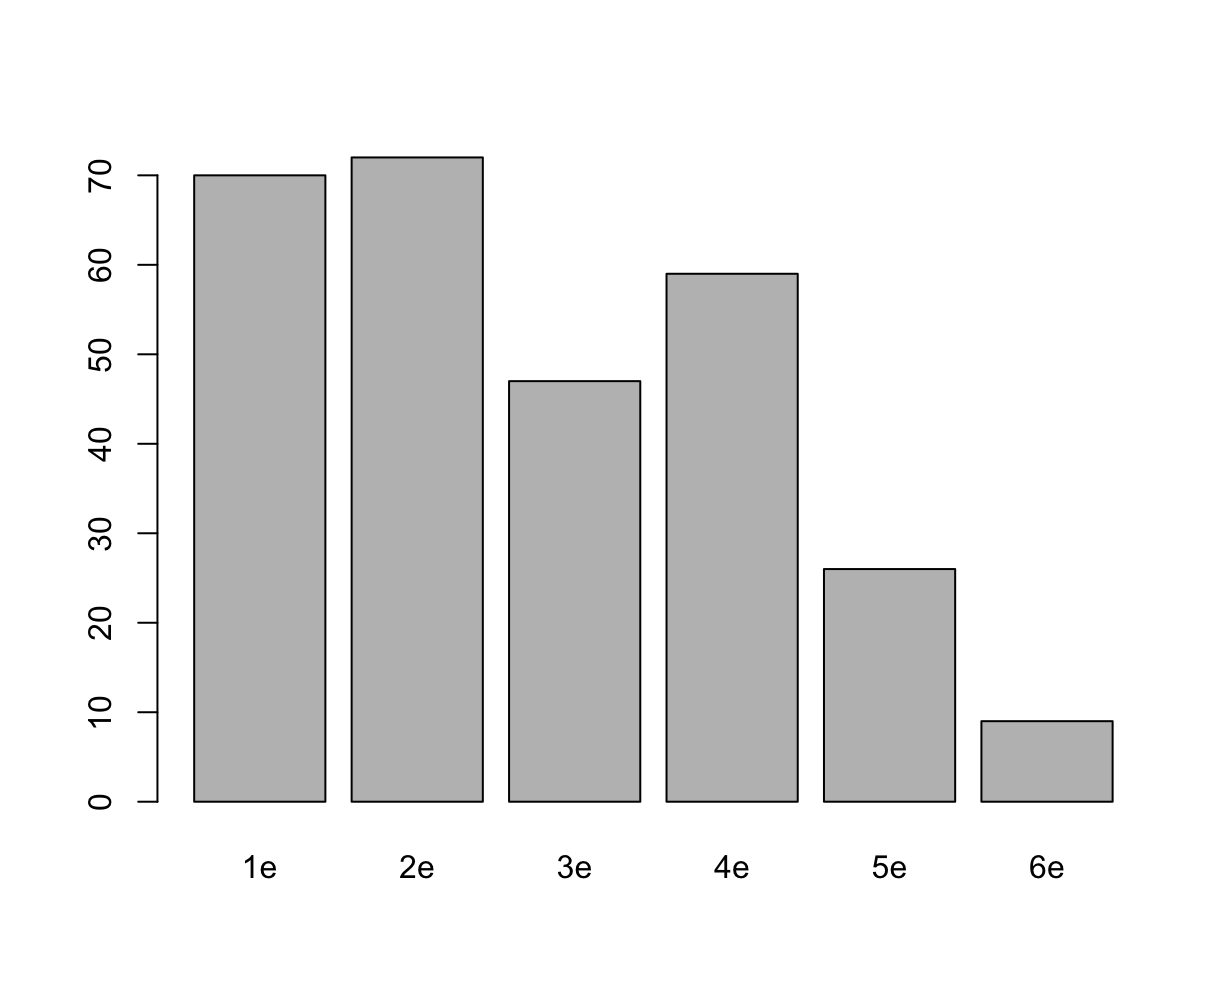
\includegraphics[width=0.5\textwidth]{Verdeling klassen.png}
    \caption{De verdeling van de respondenten tussen de jaren. (NA = 54)}
    \label{fig:verdeling}
    \end{figure}

Je ziet in figuur \ref*{fig:verdeling} dat de meeste respondenten uit de onderbouw komen. Jaar 5 en 6 zijn zelfs slecht vertegenwoordigd. Mogelijke verklaring is dat de vragenlijst in maart is afgenomen en deze leerlingen al veelal met examenvoorbereidingen bezig waren en hun laatste schooldag in zicht kwam waardoor ze misschien minder het gevoel hadden dat ze iets aan dit onderzoek zouden hebben. Het reproduceren speelt in het examenjaar waarschijnlijk ook minder een rol, hoewel ik op verzoek lijsten van veelvoorkomende signaalwoorden voor het eindexamen Frans en Duits op de SlimStampen-omgeving van het Metis Montessori Lyceum heb gezet. Van jaar 4 zijn de leerlingen weer iets meer vertegenwoordigd, dat kan komen omdat de vakken Duits, Frans en Engels in dat jaar heel actief bezig zijn met SlimStampen in de lessen. 

\begin{figure}[h]
        \centering
        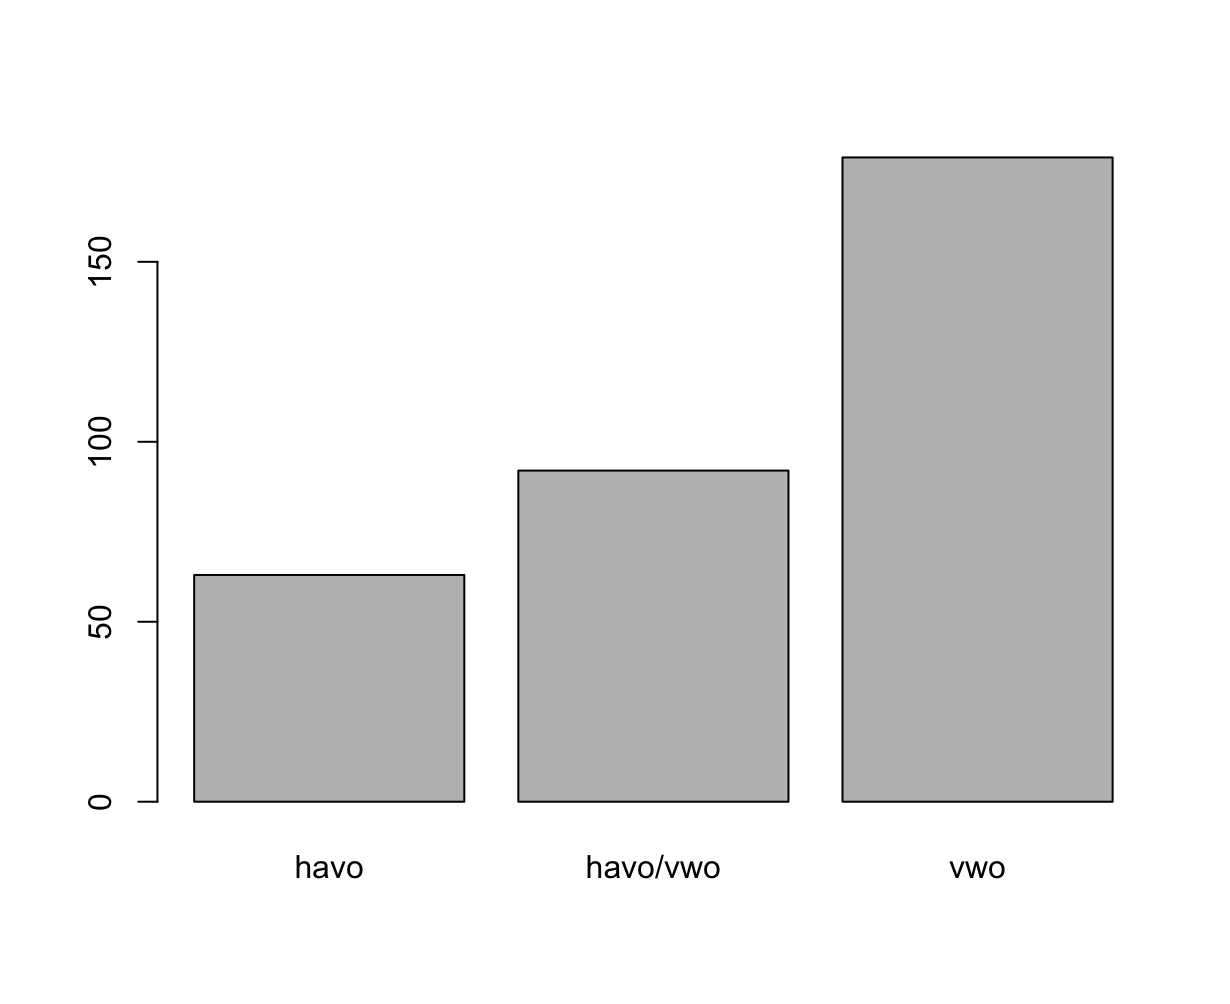
\includegraphics[width=0.5\textwidth]{niveau.png}
        \caption{Het huidige niveau van de respondenten. (NA = 3)}
        \label{fig:niveau}
        \end{figure}

Als we kijken naar niveau dan zien we in figuur \ref*{fig:niveau} dat het grootst gedeelte van de respondenten VWO niveau doet. Dit zou kunnen duiden op een grotere motivatie en betrokkenheid bij VWO leerlingen dan HAVO leerlingen. Maar we hebben een 2-jarige brugklas HAVO/VWO daar zitten ook al veel mogelijk HAVO leerlingen in. We zouden het aantal HAVO leerlingen ook wel bij de HAVO/VWO kunnen optellen dan wordt de verhouding veel kleiner (155 HAVO en 179 VWO).

\begin{figure}[h]
    \centering
    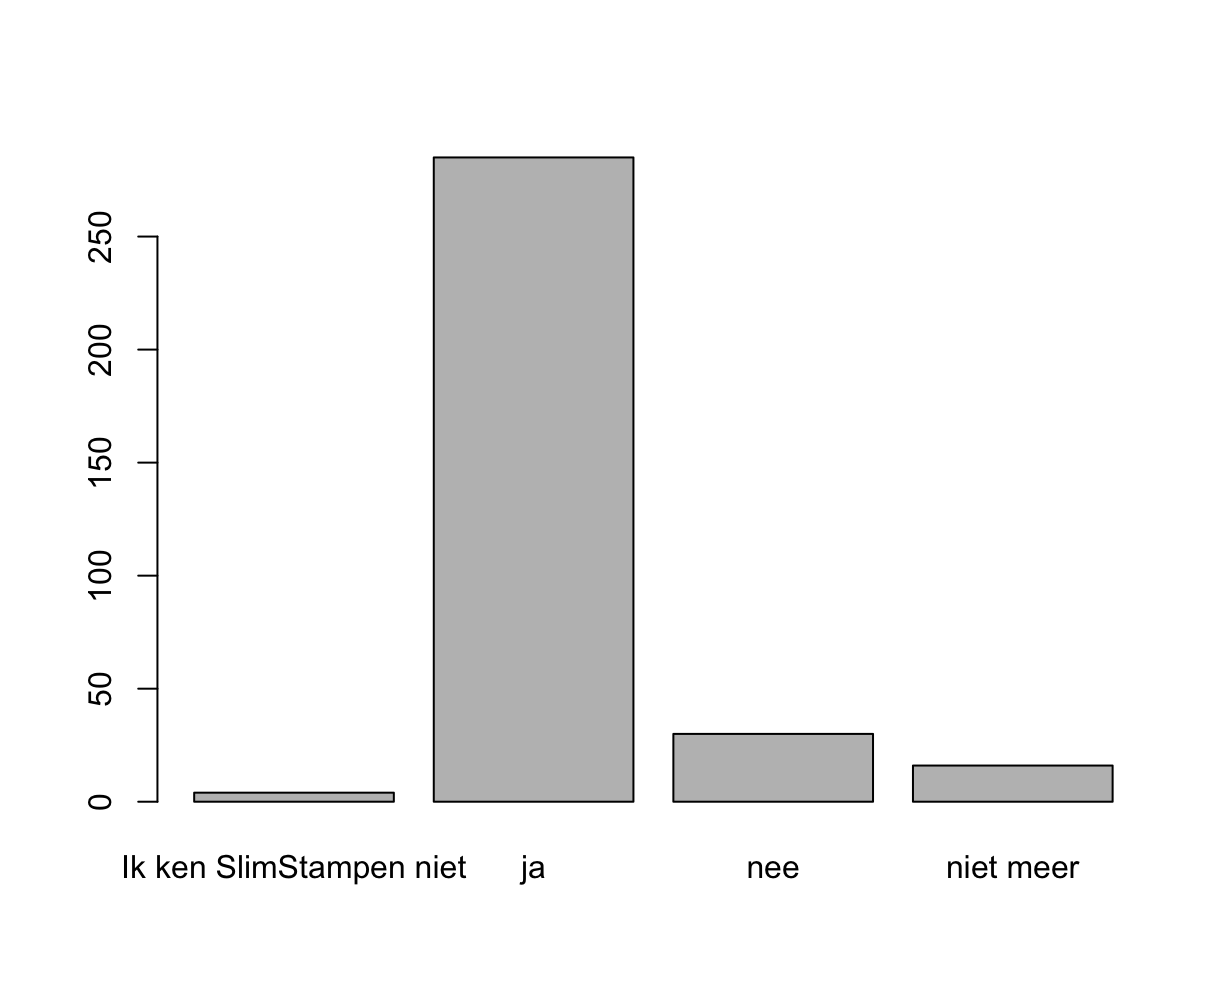
\includegraphics[width=0.5\textwidth]{kenJeSlimstampen.png}
    \caption{Gebruik je SlimStampen? (NA = 2)}
    \label{fig:kenJeSlimstampen}
    \end{figure}
Op de vraag of de respondenten SlimStampen gebruiken antwoorden 285 respondenten bevestigend. Zestien respondenten gebruikt het niet meer, dertig respondenten gebruiken het niet en 4 geven aan dat ze er nog nooit van hebben gehoord. (zie figuur \ref*{fig:kenJeSlimstampen}) Als de leerlingen SlimStampen niet (meer) gebruikten kwamen respondenten direct naar de slotvragen. Hierdoor zijn er bij de directe vragen over SlimStampen rond de 285 antwoorden.

De leerlingen moesten antwoorden op stellingen met een cijfer van 1 tot 10, waarbij 1=helemaal niet en 10=helemaal wel. Er zijn een paar open vragen.

\subsection{Voorbereide omgeving}
\begin{figure}
    \begin{tabular}{cc}
      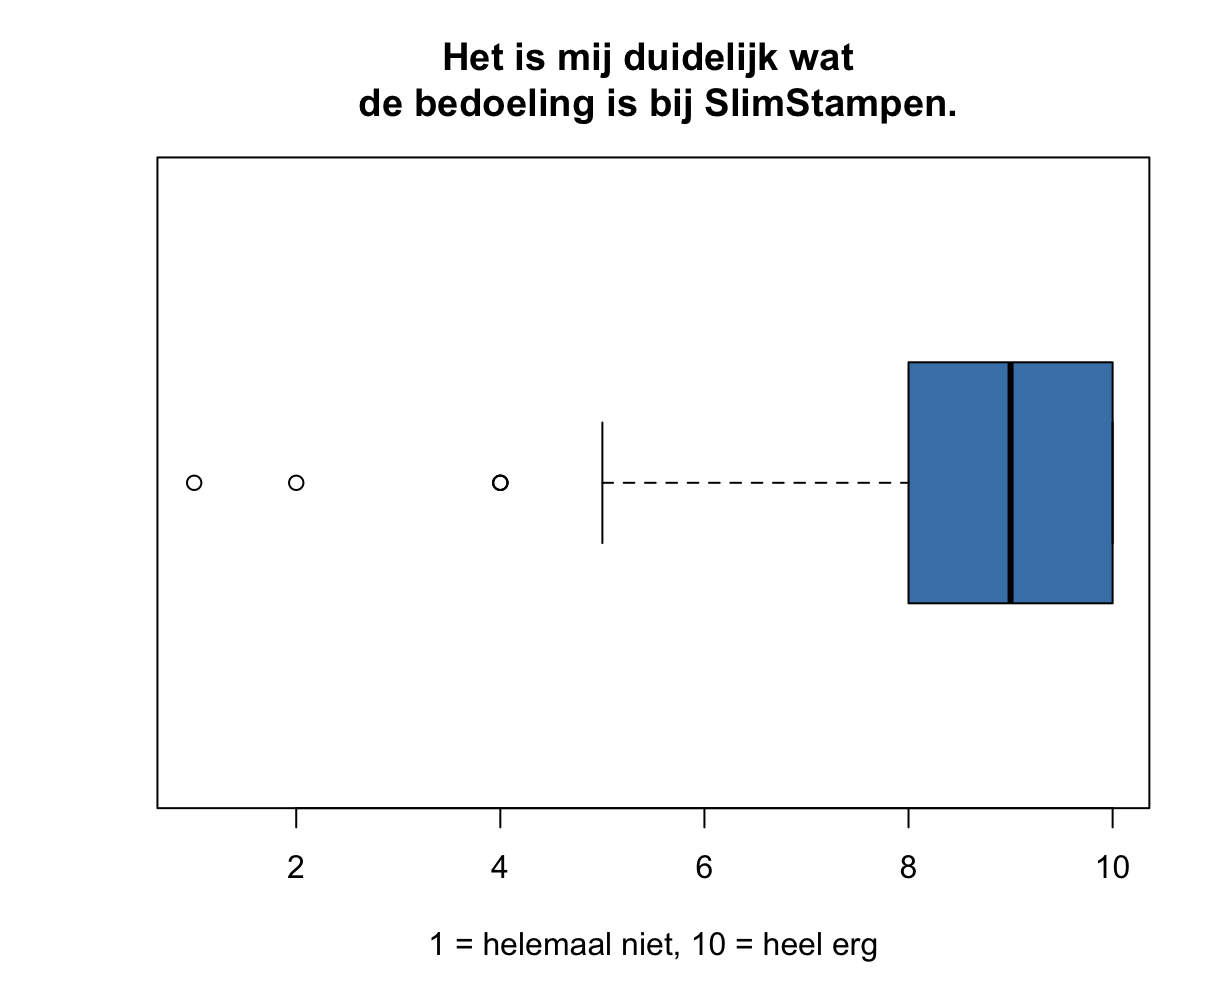
\includegraphics[width=65mm]{12-SlimStampenIsDuidelijk.png} &   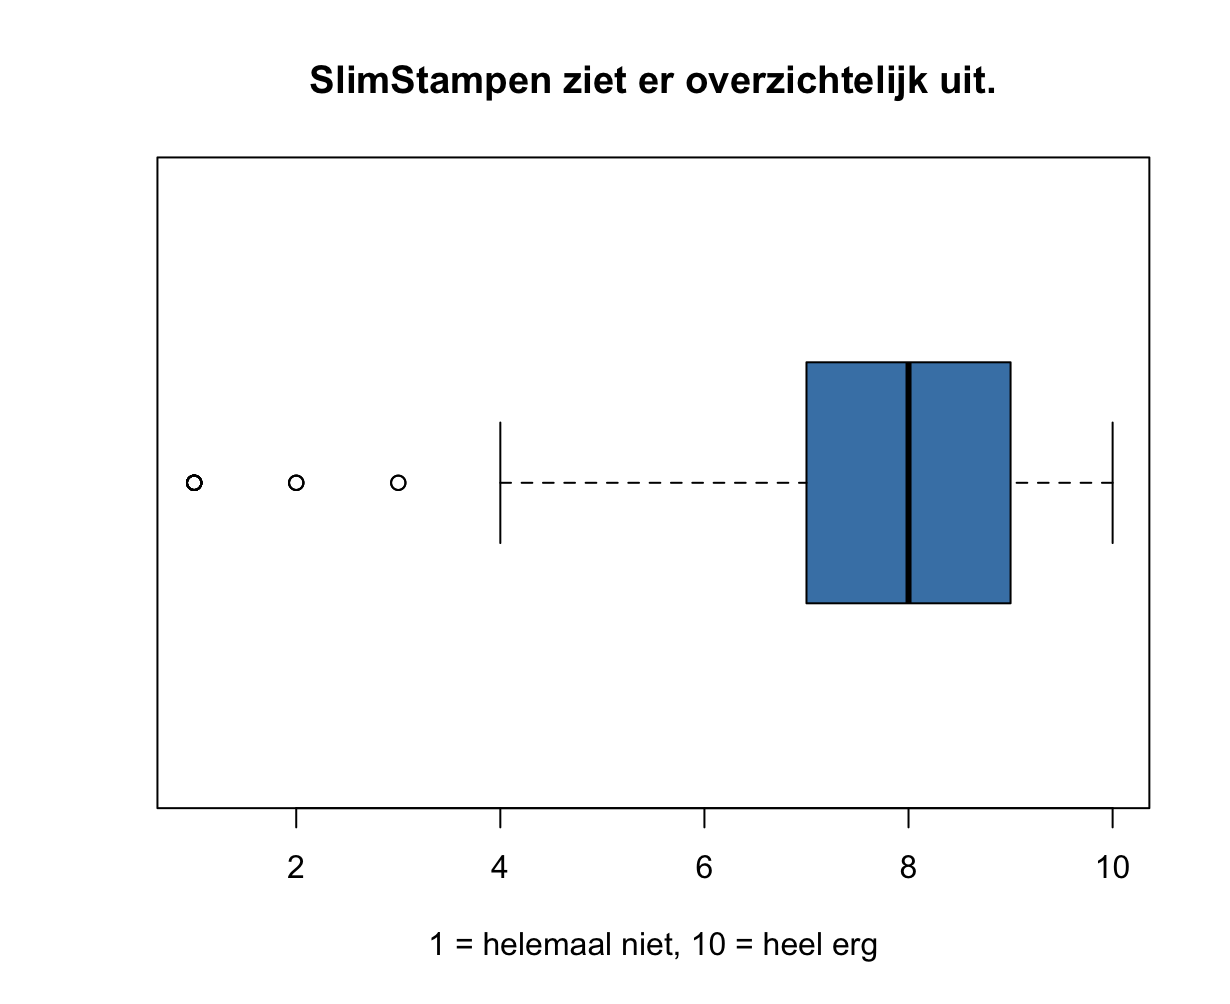
\includegraphics[width=65mm]{14-Overzichtelijk.png} \\
    (a)  $\overline{X}$ = 8.554, N=285, NA = 52 & (b) $\overline{X}$ = 7.663, N=285, NA = 52 \\[6pt]
    \end{tabular}
    \caption{indicatoren voor de voorbereide omgeving}
    \label{fig:omgeving}
    \end{figure}

De voorbereide omgeving is voor Montessori een breed begrip. Niet alleen de fysieke klas en het educatieve materiaal moeten op orde zijn en aan bepaalde eisen voldoen, maar ook de docent hoort bij de voorbereide omgeving. SlimStampen is als educatief materiaal dus maar een klein deel van de voorbereide omgeving. Dit onderzoek gaat daarmee dus op maar een klein gedeelte van de voorbereiding in. Met het gebruik van SlimStampen zorgt de docent dat het materiaal klaar staat. De leerlingen zijn vrij om het zelf erbij te pakken en kunnen zelfstandig met dit materiaal aan de slag op die momenten dat ze er zelf mee aan het werk willen. Ze kunnen zelf hun fouten controleren dus geheel onafhankelijk van de docent kunnen ze aan het werk. 
De resultaten laten zien dat SlimStampen als materiaal er duidelijk uitziet en leerlingen weten wat ze daar moeten doen. Op de vraag of het duidelijk is wat er met SlimStampen moet gebeuren (zie Figuur \ref*{fig:omgeving}(a)) zie je dat het eerste kwartiel al op de acht zit, het tweede kwartiel zelfs al op tien. Leerlingen weten waar dit materiaal voor bedoeld is en kunnen er mee aan de slag. Ook op de vraag of SlimStampen overzichtelijk is zijn de meeste leerlingen uitermate positief (zie Figuur \ref*{fig:omgeving}(b)). Concluderend; de leerlingen zijn positief over het materiaal op zich.

\subsection{Normalisatie}
\begin{figure}
    \begin{tabular}{cc}
      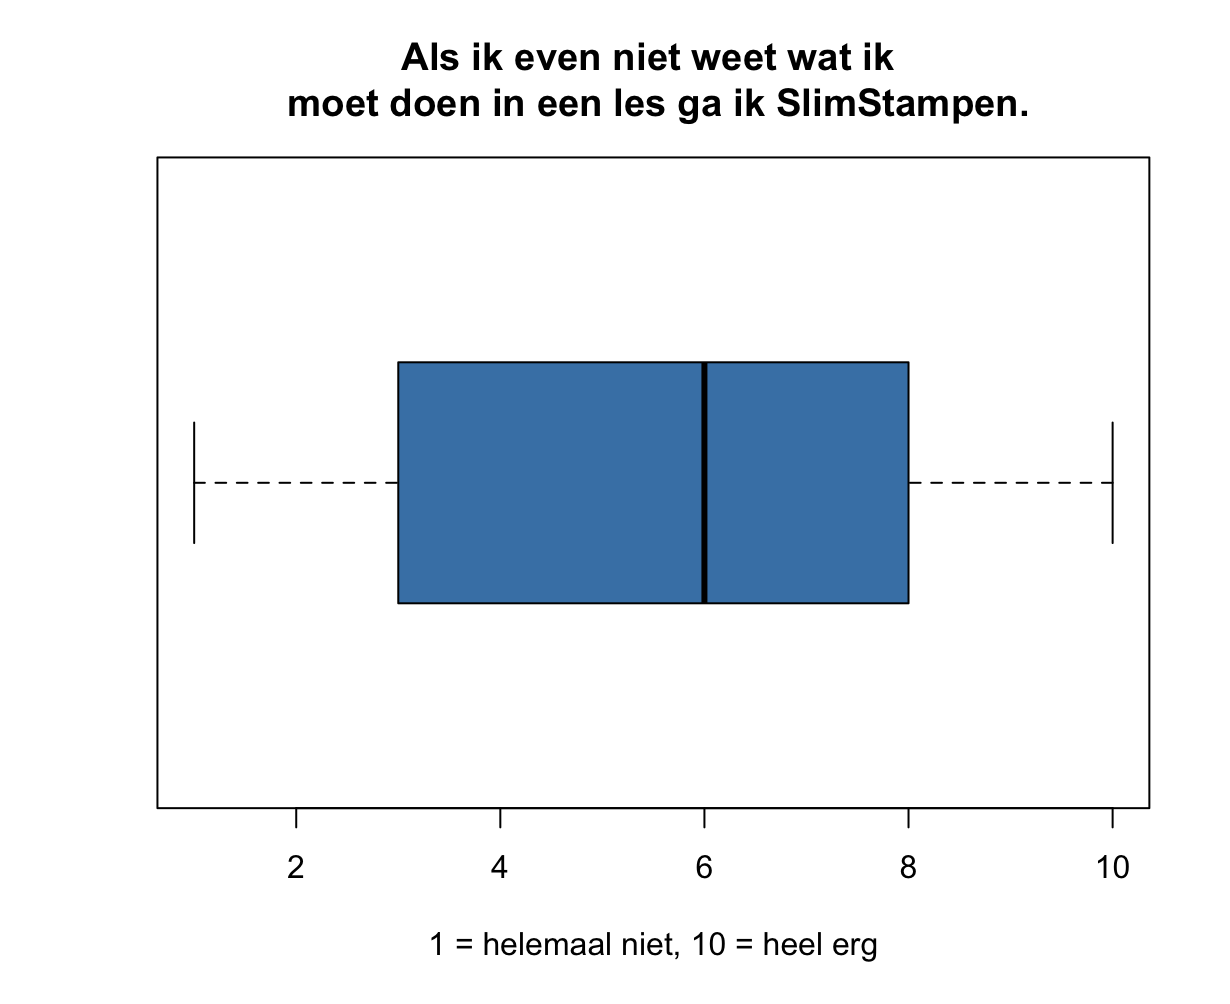
\includegraphics[width=65mm]{11-AlsIkNietWeetGaSlimstampen.png} &   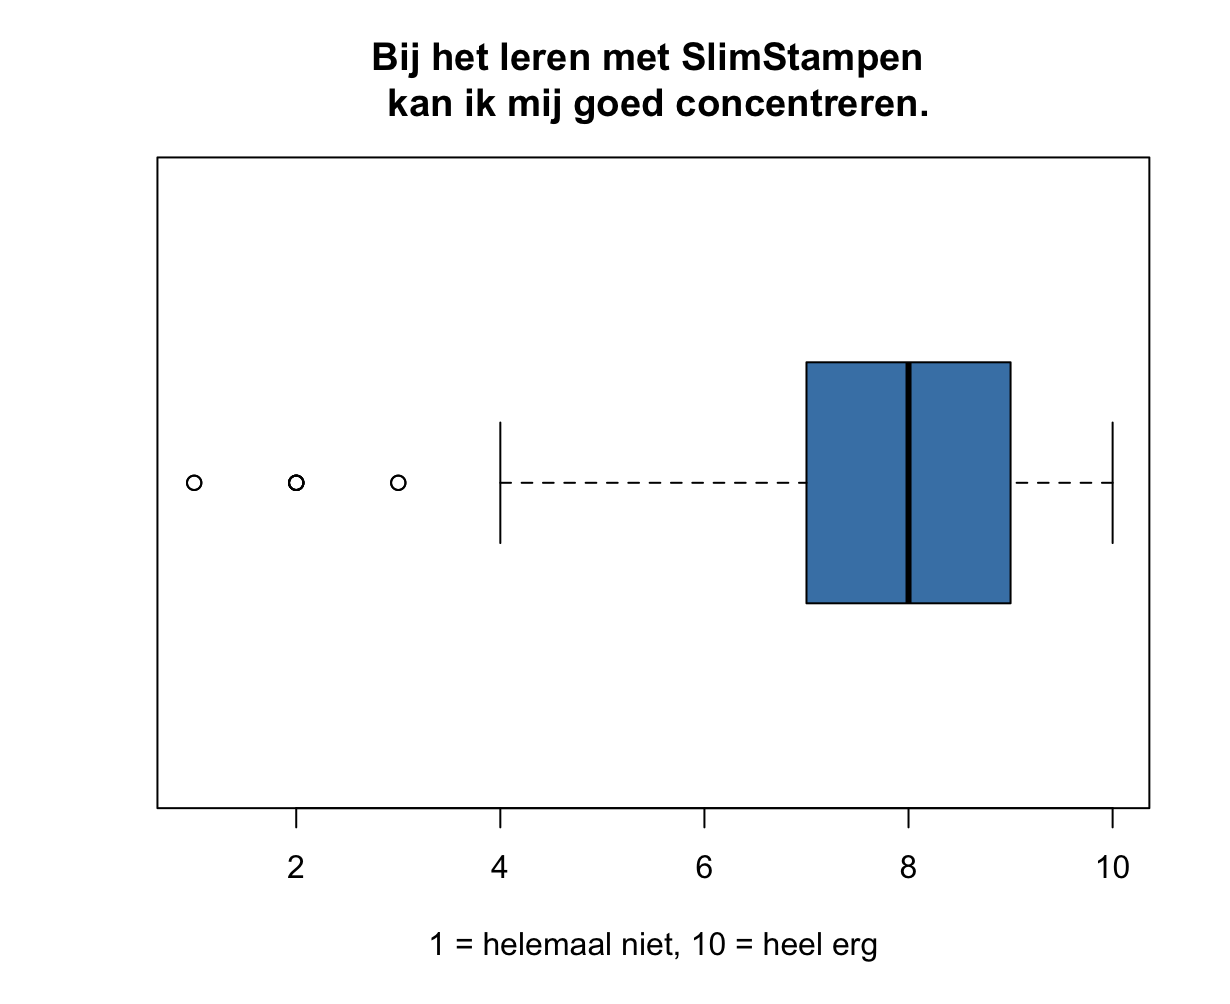
\includegraphics[width=65mm]{13-ConcentratieBijSlimStampen.png} \\
    (a)  $\overline{X}$ = 5.568, N=285, NA = 52 & (b) $\overline{X}$ = 7.616, N=284, NA = 53 \\[6pt]
     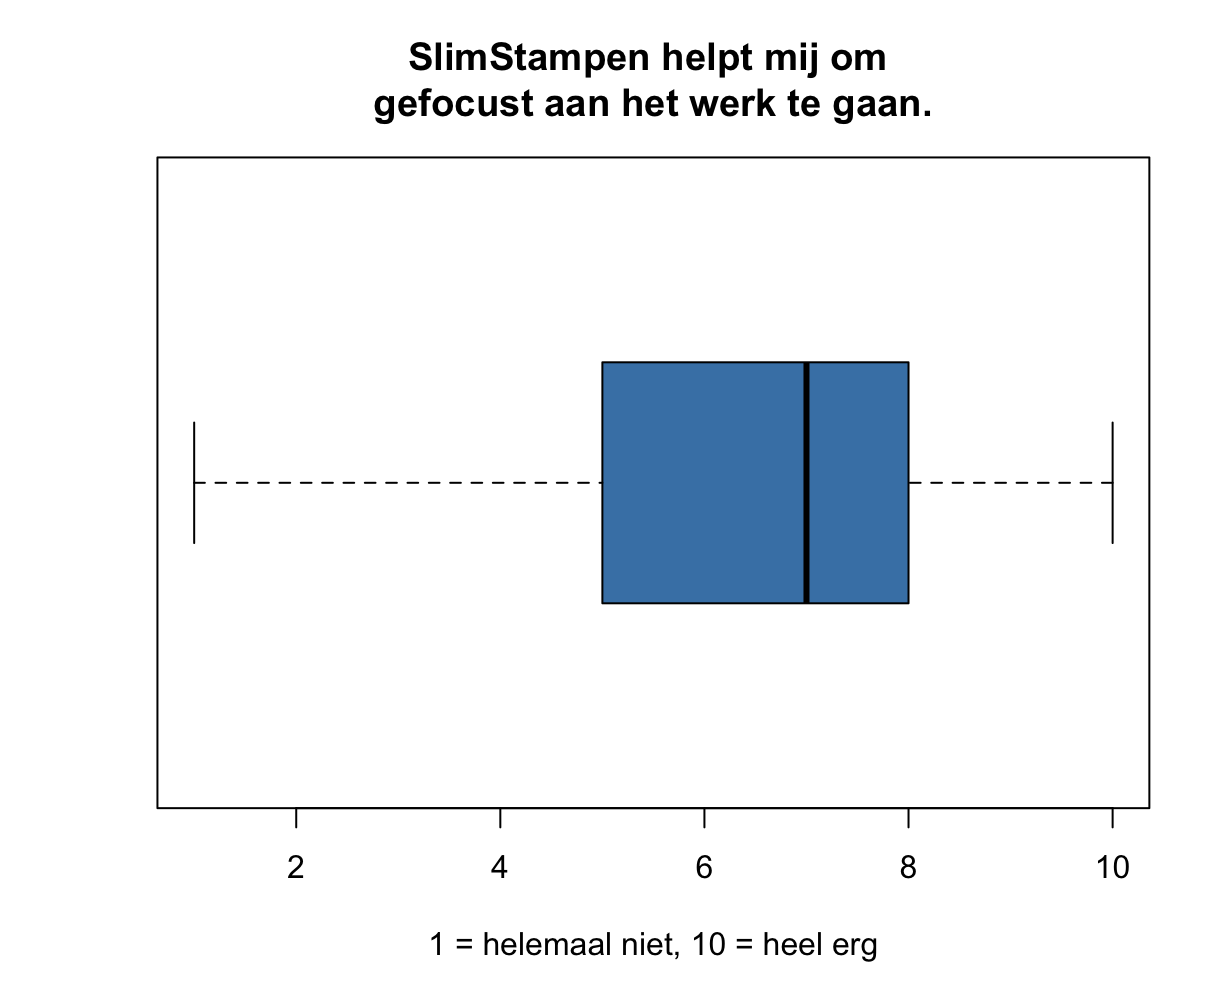
\includegraphics[width=65mm]{17-GefocustAanHetWerk.png} &   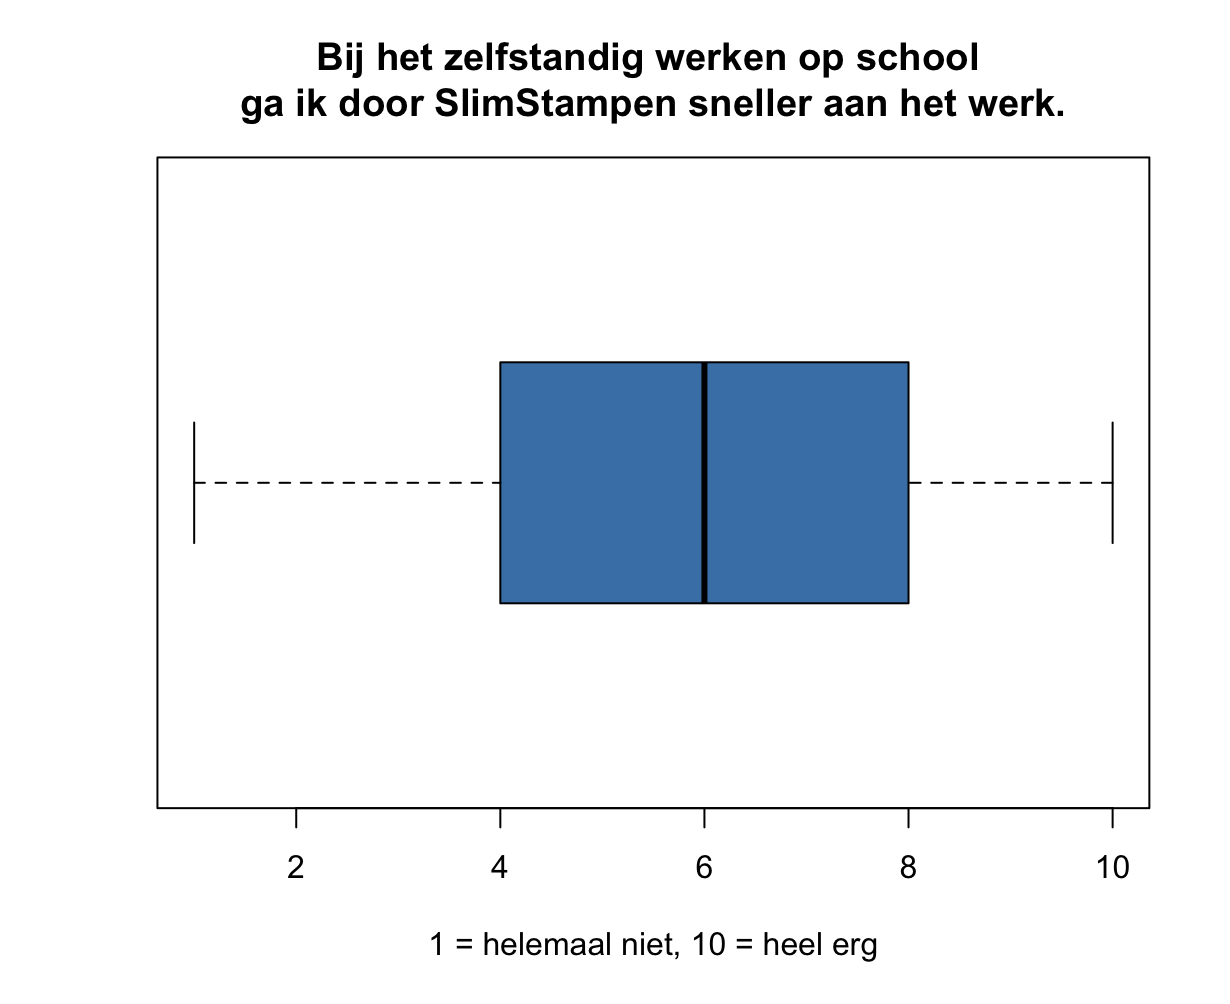
\includegraphics[width=65mm]{18-SnellerAanHetWerk.png} \\
    (c) $\overline{X}$ = 6.553, N=284, NA = 53 & (d) $\overline{X}$ = 6.018, N=284, NA = 53 \\[6pt]
    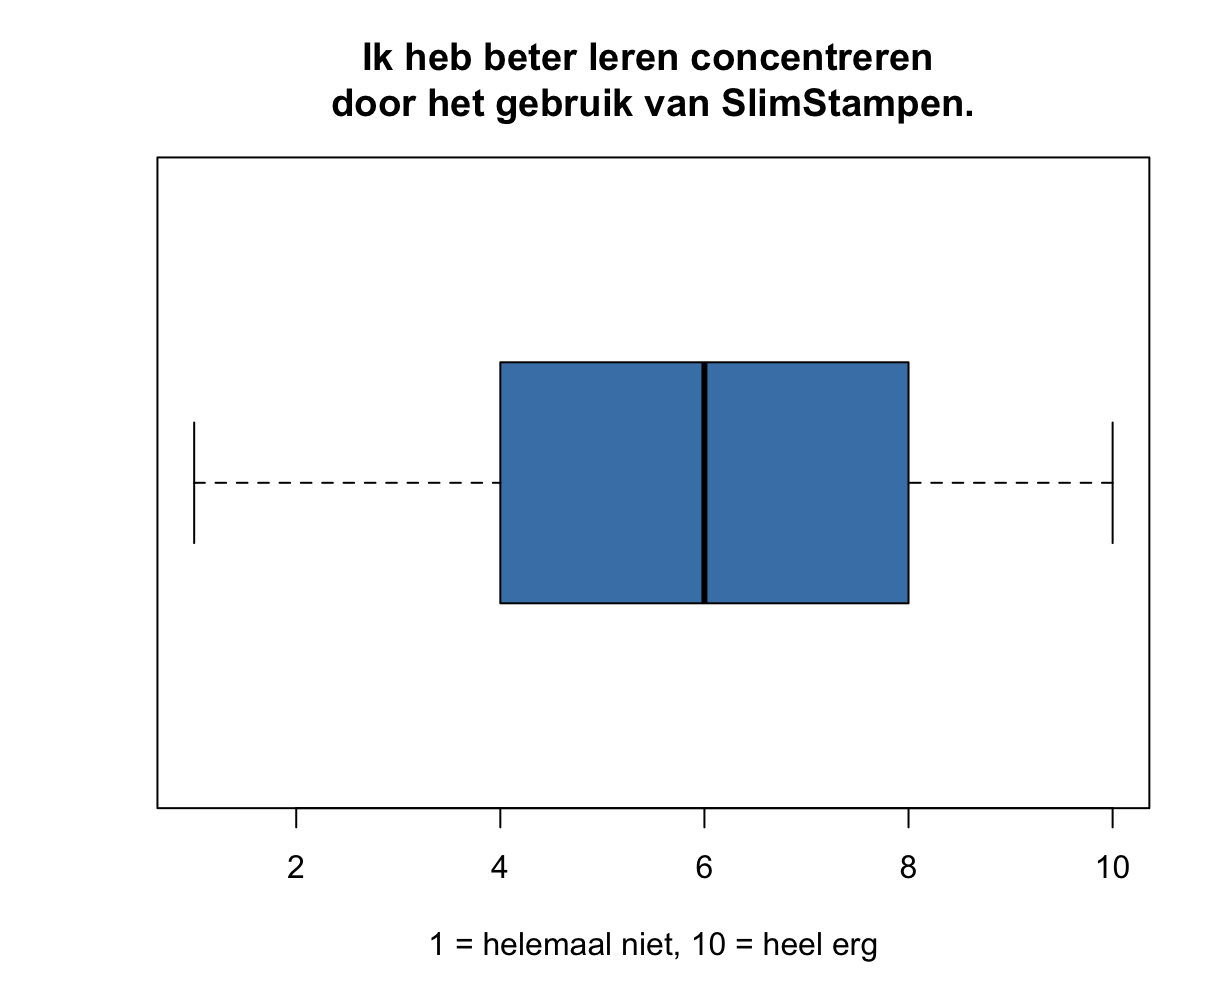
\includegraphics[width=65mm]{28-BeterLerenConcentreren.png} & 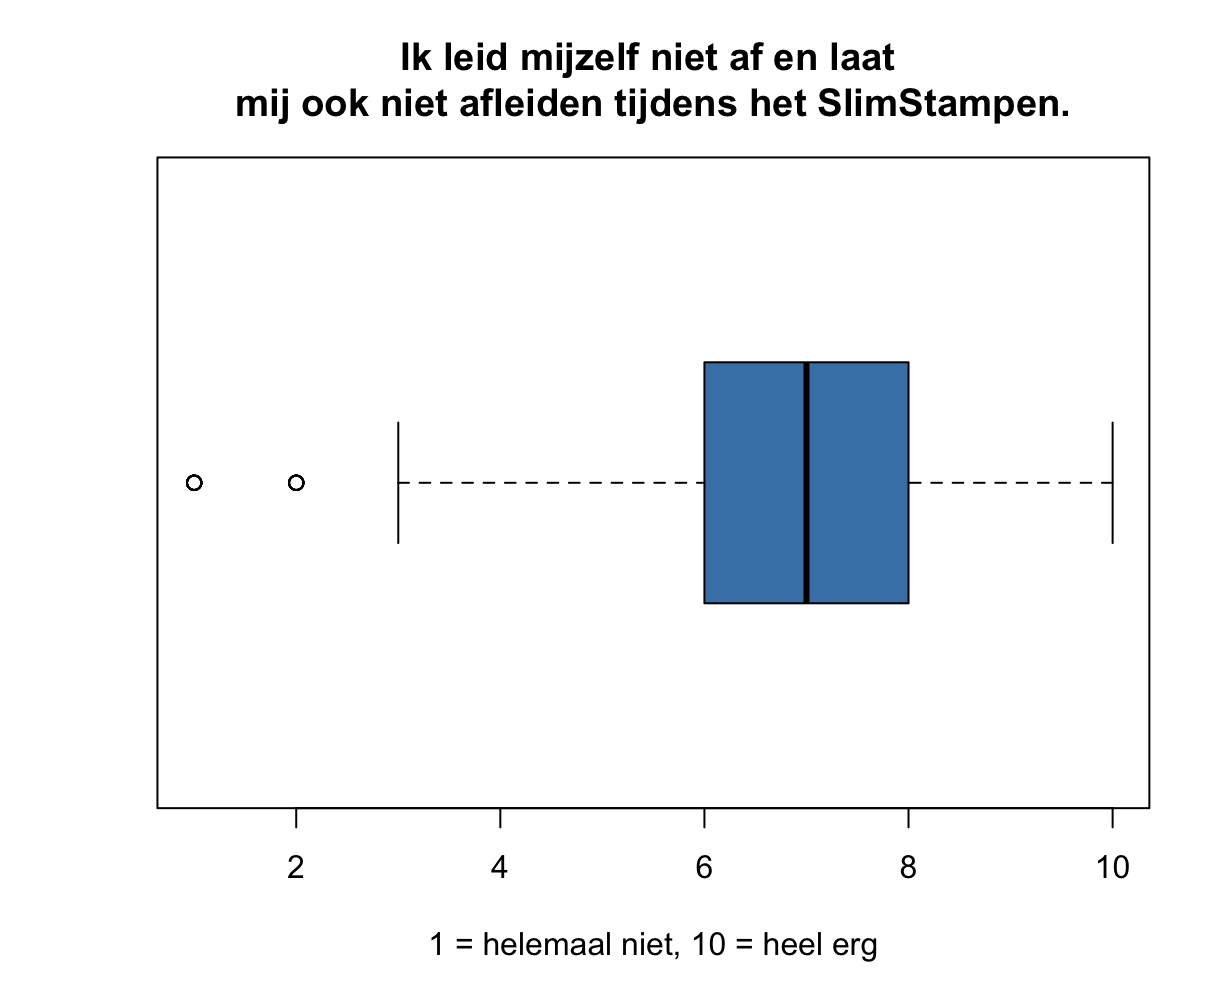
\includegraphics[width=65mm]{images/15-LaatNietAfleiden.png}\\
    (e) $\overline{X}$ = 5.879, N=281, NA = 56 & (f) $\overline{X}$ = 6.705, N=285, NA = 52  
    \end{tabular}
    \caption{indicatoren voor betere normalisatie}
    \label{fig:normalisatie}
    \end{figure}
De normalisatie van de leerling is moeilijk te meten en kan je op veel manieren interpreteren. Voornamelijk door te observeren kan je waarnemen of een leerling 'genormaliseerd' is. Een leerling kan zelfstandig aan het werk beginnen en kan zichzelf in een diepere concentratie brengen, zonder dat de docent nodig is. Normalisatie raakt de taakaanvaarding van de leerling. Helpt SlimStampen bij de concentratie en komt een leerling sneller aan het werk door SlimStampen? De antwoorden op deze vragen geven een indicatie van de normalisatie van de leerling.

Uit figuur \ref*{fig:normalisatie}(a) blijkt dat veel leerlingen niet automatisch SlimStampen erbij pakken als ze even niet weten wat ze moeten doen. Mijn idee was dat SlimStampen ook gebruikt zou kunnen worden als alternatief voor ander werk. Als de leerling even niet weet wat het kan doen dat het dan makkelijk naar SlimStampen zou gaan. Deze hypothese is niet overtuigend positief. 
De leerlingen zijn overwegend positief over de concentratie die ze bereiken bij het werken met SlimStampen \ref*{fig:normalisatie}(b). Dit is ook wel nodig, omdat het leeralgoritme rekening houdt met de reactietijd. 

SlimStampen helpt veel leerlingen om gefocust aan het werk te gaan. Dit past goed bij wat Maria Montessori zag als normalisatie. Dit is ook mijn ervaring tijdens mijn observatie; als leerlingen beginnen in het lesuur met SlimStampen komen ze snel in de 'leermodus' (zie figuur \ref*{fig:normalisatie}(c)).

Of SlimStampen helpt om sneller aan het werk te gaan tijdens de les zijn de leerlingen redelijk neutraal. Ik heb wel het idee, maar dit is niet sterk terug te zien in de data (zie figuur \ref*{fig:normalisatie}(d)).
Ik had gehoopt dat leerlingen het belang van concentratie zouden ervaren met het gebruik van SlimStampen en dit ook zouden leren door het gebruik. Dit blijkt niet direct uit figuur \ref*{fig:normalisatie}(e). In ieder geval geven ze aan niet direct beter \emph{te leren} concentreren. 
Figuur \ref*{fig:normalisatie}(f) laat zien dat leerlingen zich niet snel laten afleiden bij het SlimStampen en zichzelf ook niet afleiden. Aannemelijk is (zie ook figuur \ref*{fig:normalisatie}(b)) dat zij onbewust de staat van diepe concentratie bereiken tijdens het werken met SlimStampen.

\subsection{Motivatie}
\begin{figure}
    \begin{tabular}{cc}
      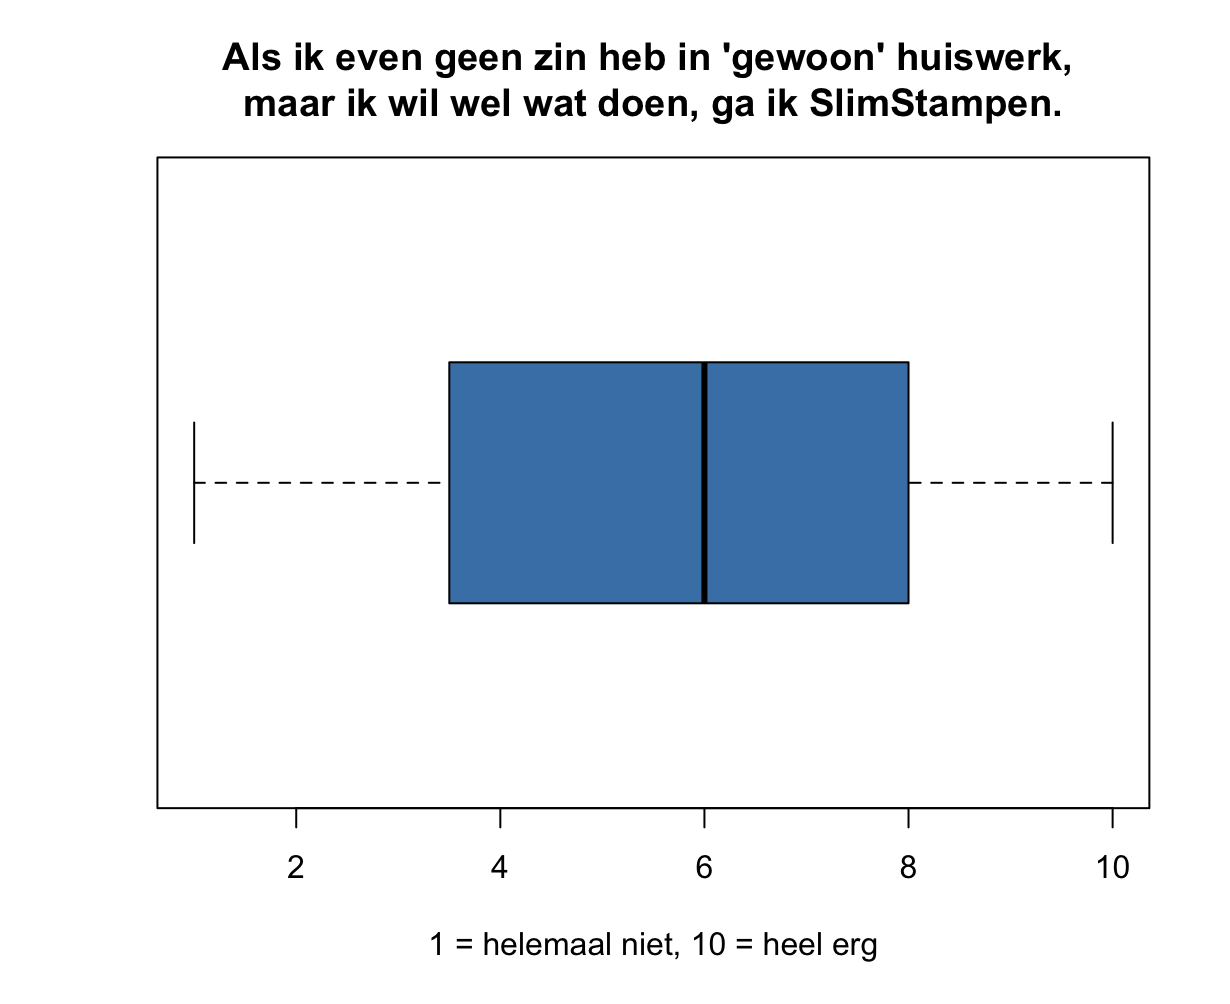
\includegraphics[width=65mm]{images/16-TwijfelGaIkSlimStampen.png} &   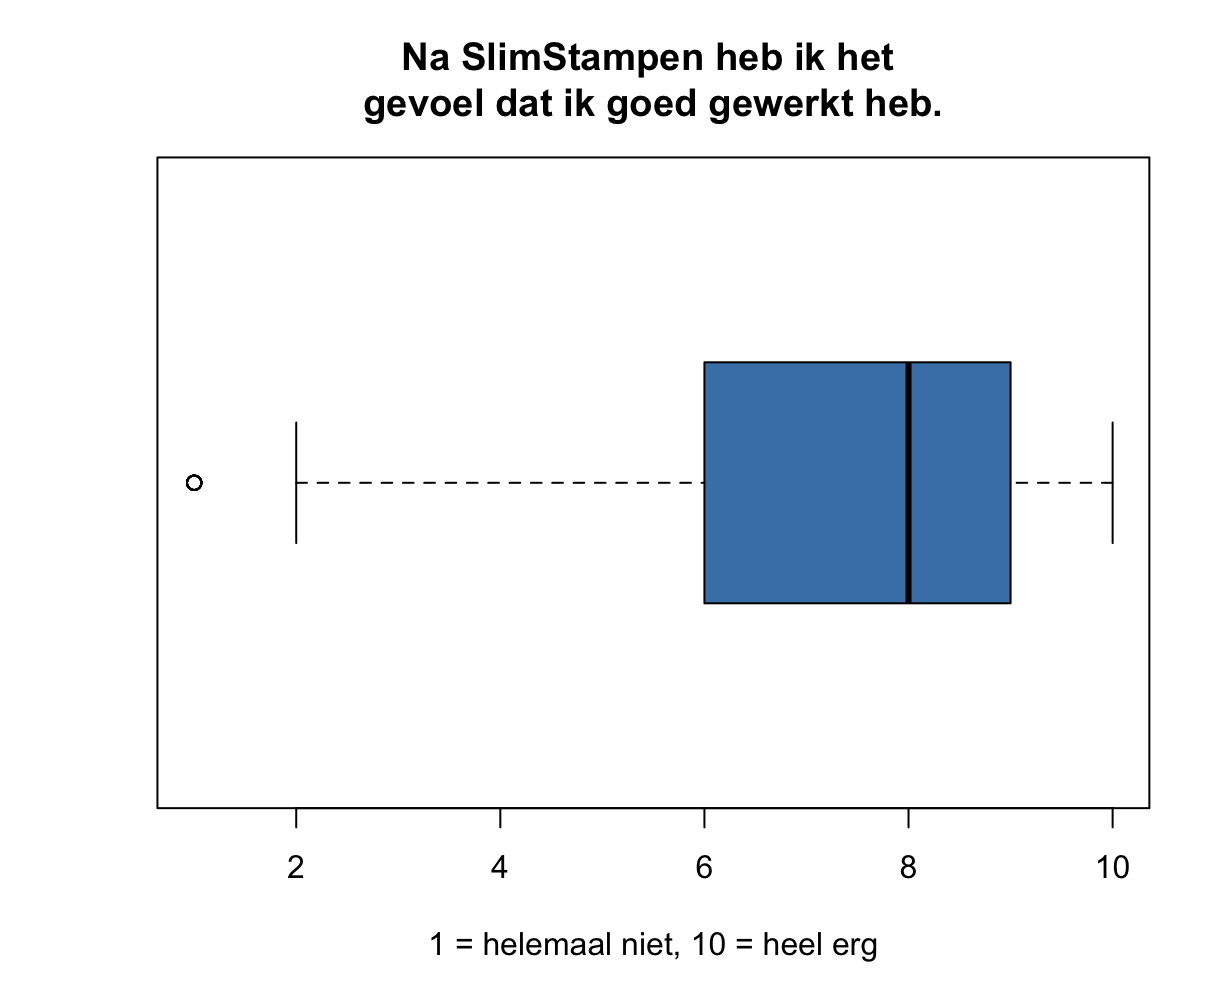
\includegraphics[width=65mm]{images/19-GevoelGoedGewerkt.png} \\
    (a) $\overline{X}$ = 5.855, N=283, NA = 54   & (b) $\overline{X}$ = 7.34, N=285, NA = 52  \\[6pt]
     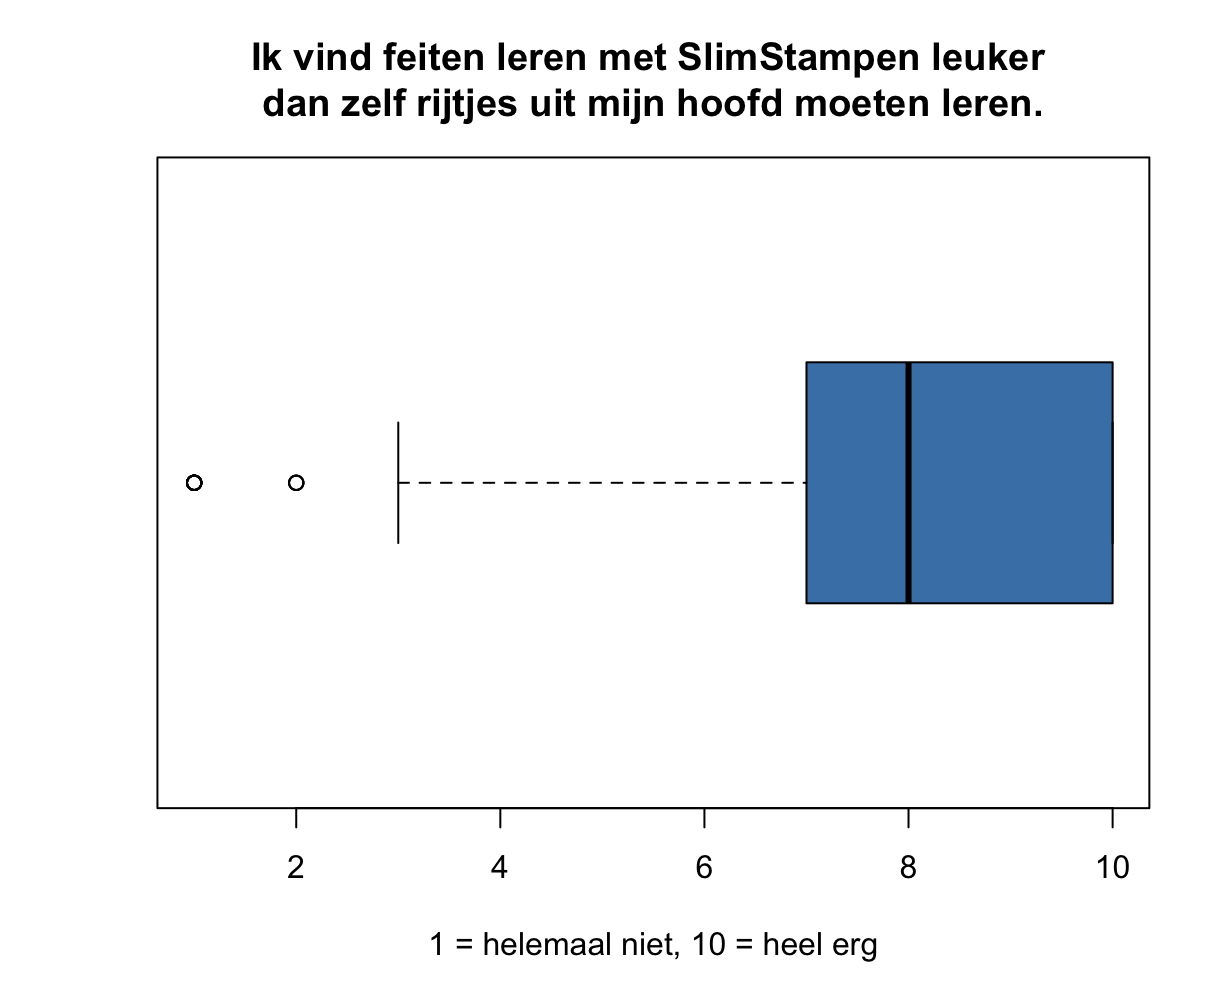
\includegraphics[width=65mm]{images/20-SlimStampenLeukerDanRijtjes.png} &   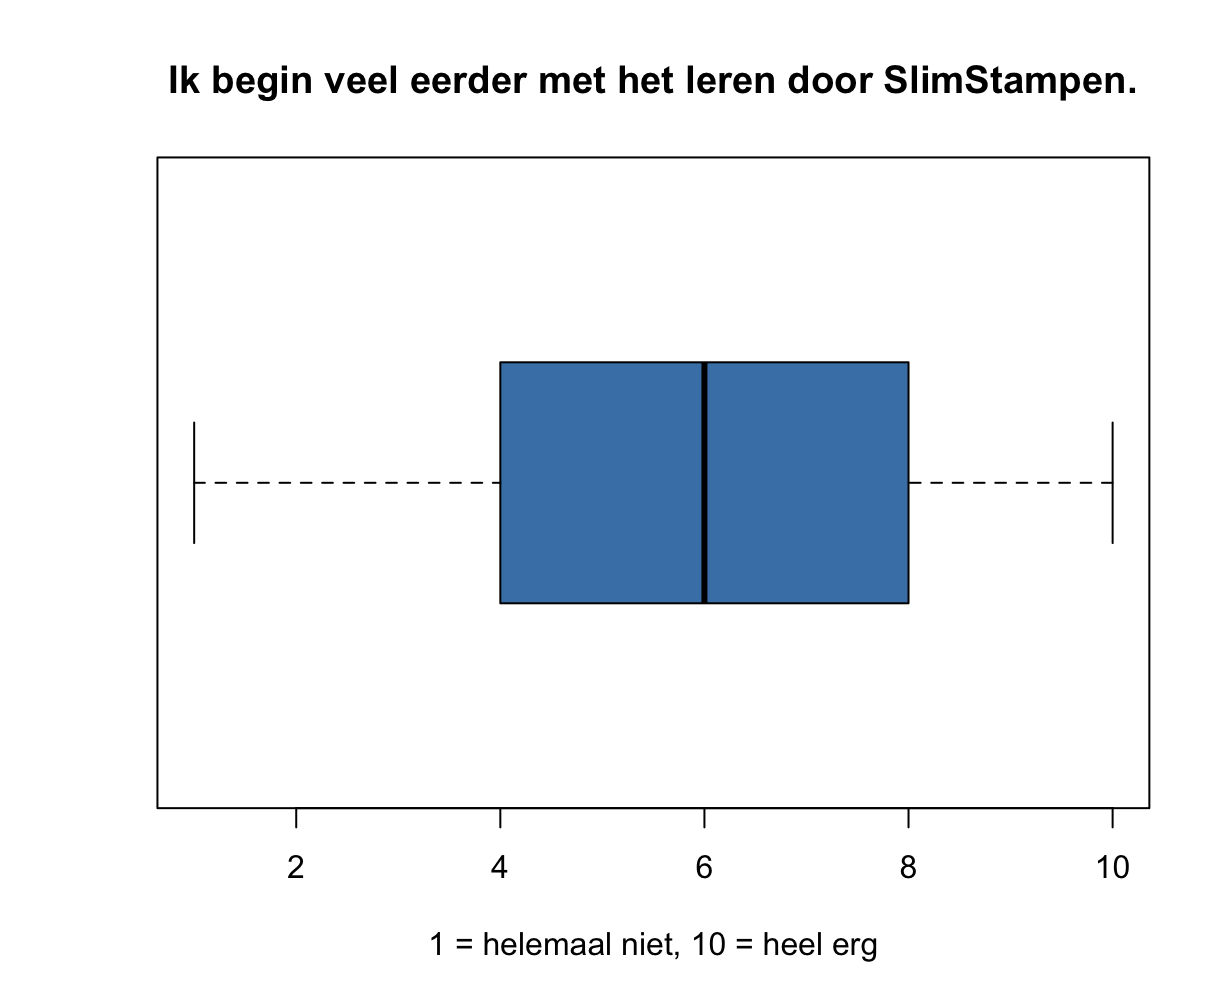
\includegraphics[width=65mm]{images/21-BeginEerder.png} \\
    (c) $\overline{X}$ = 7.818, N=280, NA = 57  & (d) $\overline{X}$ = 6.163, N=283, NA = 54  \\[6pt]
    \multicolumn{2}{c}{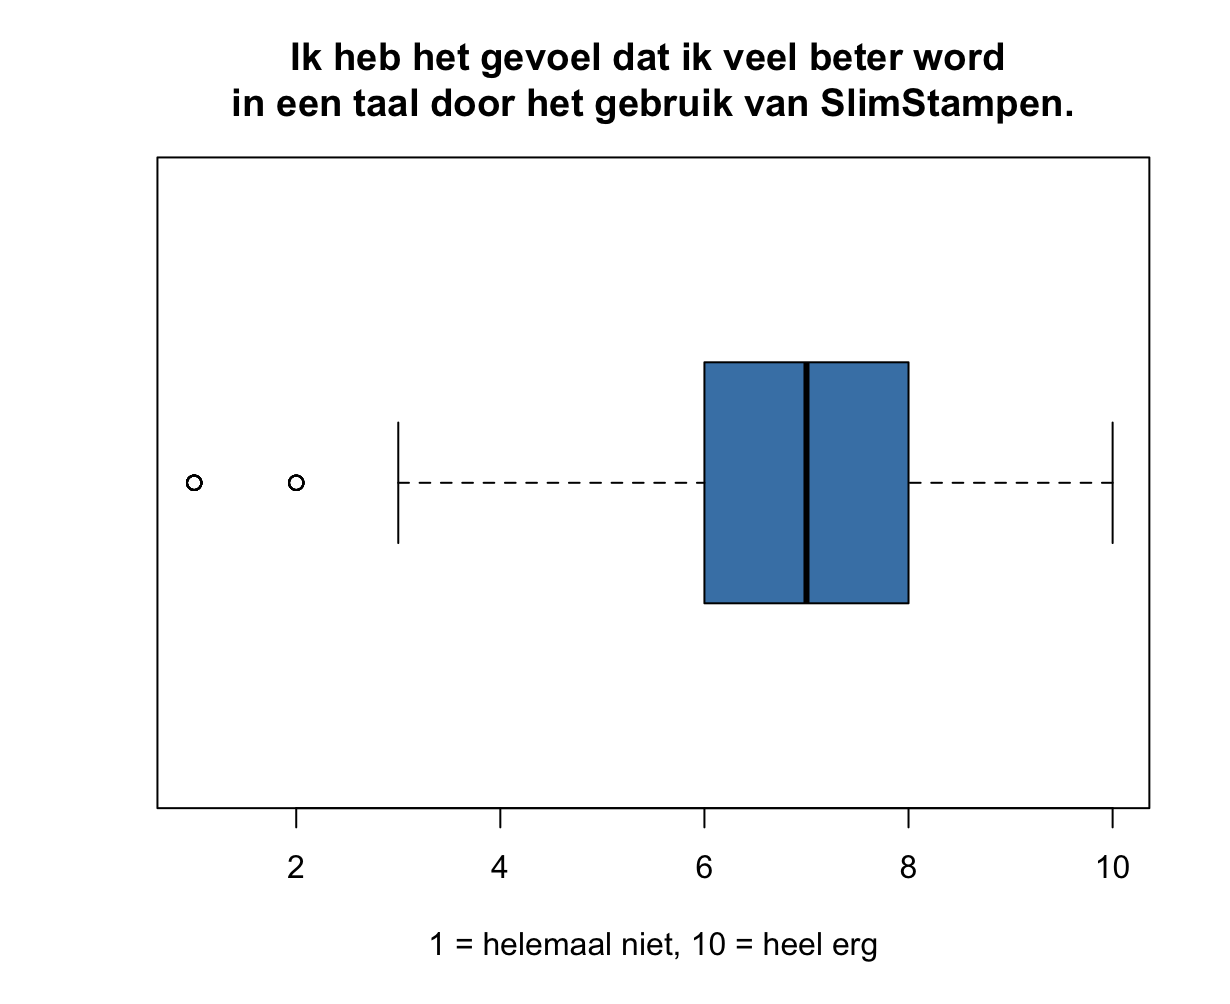
\includegraphics[width=65mm]{23-BeterInTaal.png} }\\
    \multicolumn{2}{c}{(e) $\overline{X}$ = 6.852, N=283, NA = 54}
    \end{tabular}
    \caption{indicatoren voor hogere motivatie}
    \label{fig:motivatie}
    \end{figure}

Maria Montessori ging uit van de intrinsieke motivatie van de leerling. Kinderen hebben een absorberende geest en willen leren. Tieners zijn voorbij deze gevoelige periode voor het absorberen van kennis. De ontwikkeling van de persoonlijkheid en als individu is in deze fase belangrijker. Toch is het bijbrengen van kennis een van de doelen van het onderwijs, ook in het voortgezet onderwijs. Dit lukt alleen als de leerling enigszinds gemotiveerd is, intrinsiek of extrensiek. Volgens de zelfdeterminatietheorie van Deci en Ryan hebben leerlingen drie basisbehoeften: autonomie, competentie en verbondenheid. Als deze behoeften vervuld zijn, is de kans een stuk groter dat de leerling gemotiveerd is \cite[p.436-439]{woolfolk}.

Zin hebben in iets is een vorm van intrinsieke motivatie. Ook al is het soms voor een leerling een keuze tussen twee kwaden. SlimStampen is niet zo moeilijk in die zin dat het simpelweg ''stampen'' is. Er worden geen hogere denkvaardigheden aangesproken. Verstand op nul en aan het werk. Ik was benieuwd of leerlingen SlimStampen ook zo zouden zien. Niet zo'n zin in hogere denkvaardigheden, maar wel energie genoeg om te SlimStampen. Deze hypothese wordt niet door alle leerlingen gedeeld. Ze staan hier licht positief tegenover, maar een groot gedeelte ook niet (zie figuur \ref*{fig:motivatie}(a)).
Een positief gevoel nadat je gewerkt hebt levert je motivatie op voor een volgende keer. Geeft het leren met SlimStampen een positief gevoel achteraf? Hier zijn de meeste leerlingen het wel over eens. In figuur \ref*{fig:motivatie}(b) is duidelijk te zien dat veel leerlingen het gevoel hebben goed te hebben gewerkt nadat ze hebben geoefend met SlimStampen.

Woordjes uit je hoofd leren voor een toets gebeurt vrijwel op iedere school. Het is het simpelweg stampen van kennis. Niet altijd leuk, wel noodzakelijk om bijvoorbeeld een nieuwe taal te leren. De meeste leerlingen geven aan het leren van feiten met SlimStampen veel leuker te vinden dan het leren van rijtjes. In figuur \ref*{fig:motivatie}(c) zie je dat vrijwel alle leerlingen hier positief tot zeer positief over zijn.

Op de vraag of de leerlingen veel eerder beginnen met leren door SlimStampen zijn de leerlingen redelijk normaal verdeeld. Het gemiddelde is een 6.163 net positief (zie figuur \ref*{fig:motivatie}(d)). Mijn idee met deze vraag was dat gemotiveerde leerlingen uit zichzelf eerder zullen beginnen met een taak. Met SlimStampen ben je verplicht om minstens drie dagen te leren (per dag kan je een mastery kroontje halen). Het kan dus zo zijn dat leerlingen alleen daarom eerder beginnen.

In figuur \ref*{fig:motivatie}(e) zie je dat veel leerlingen over het algemeen het idee hebben dat ze beter worden in een taal door het gebruik van SlimStampen. Dit zal ze hoogstwaarschijnlijk meer zelfvertrouwen geven om een taal te leren en waarschijnlijk daarmee ook meer motivatie.

    \begin{figure}
        \begin{tabular}{cc}
          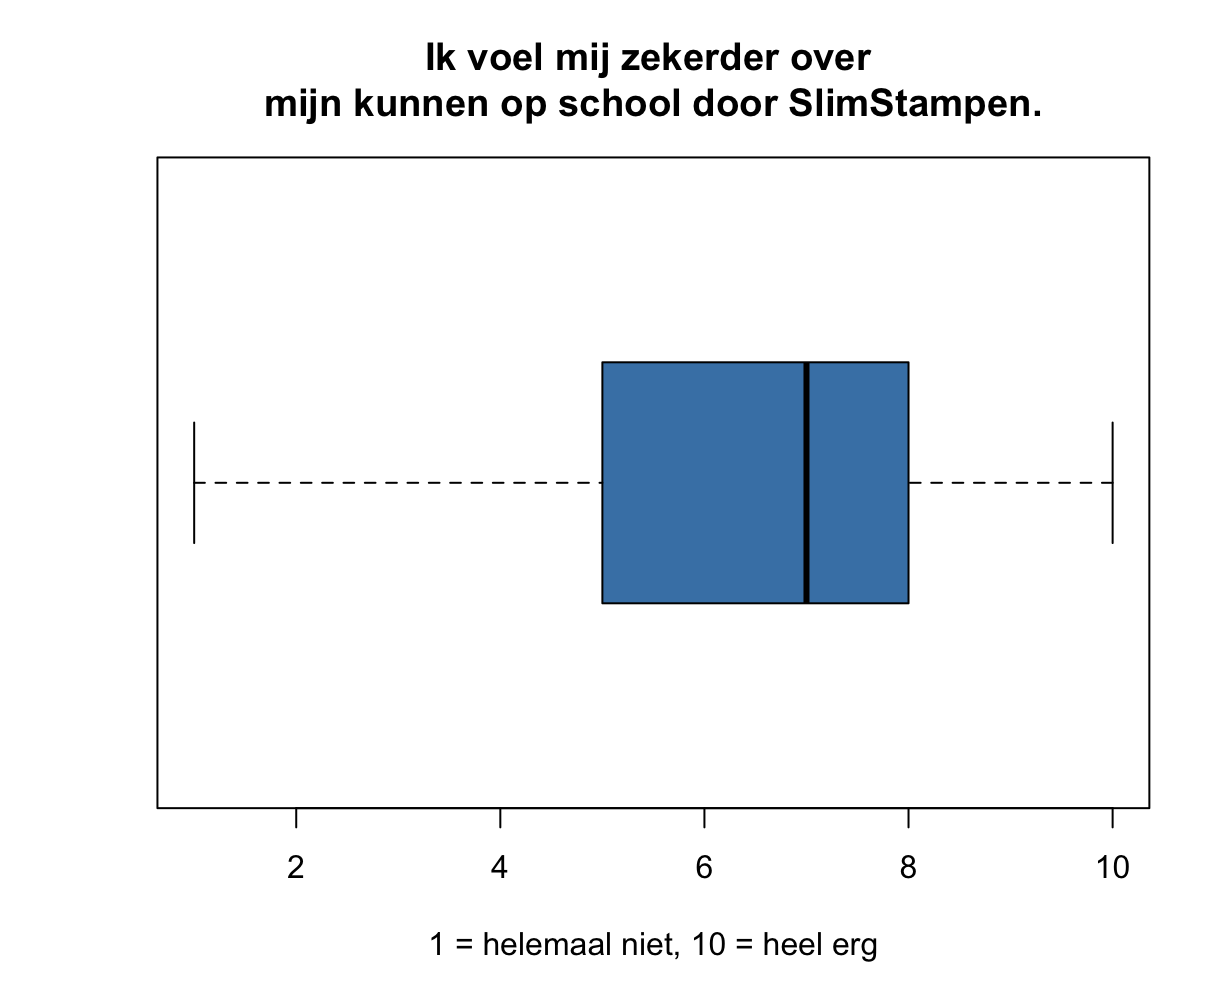
\includegraphics[width=65mm]{images/24-VoelZekerder.png} &   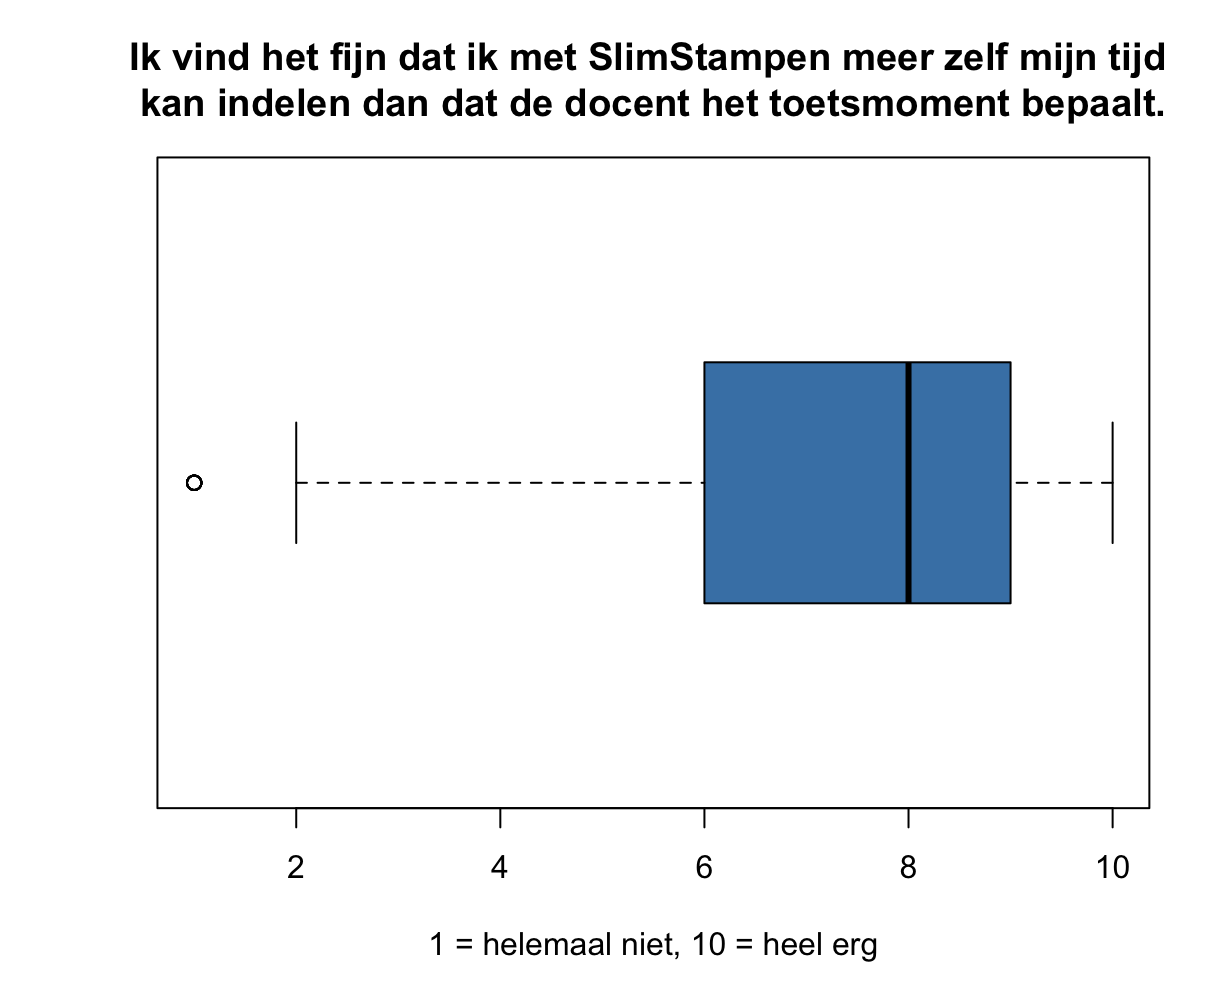
\includegraphics[width=65mm]{images/27-ZelfTijdIndelen.png} \\
        (a) $\overline{X}$ = 6.246, N=281, NA = 56   & (b) $\overline{X}$ = 7.241, N=282, NA = 55  \\[6pt]
         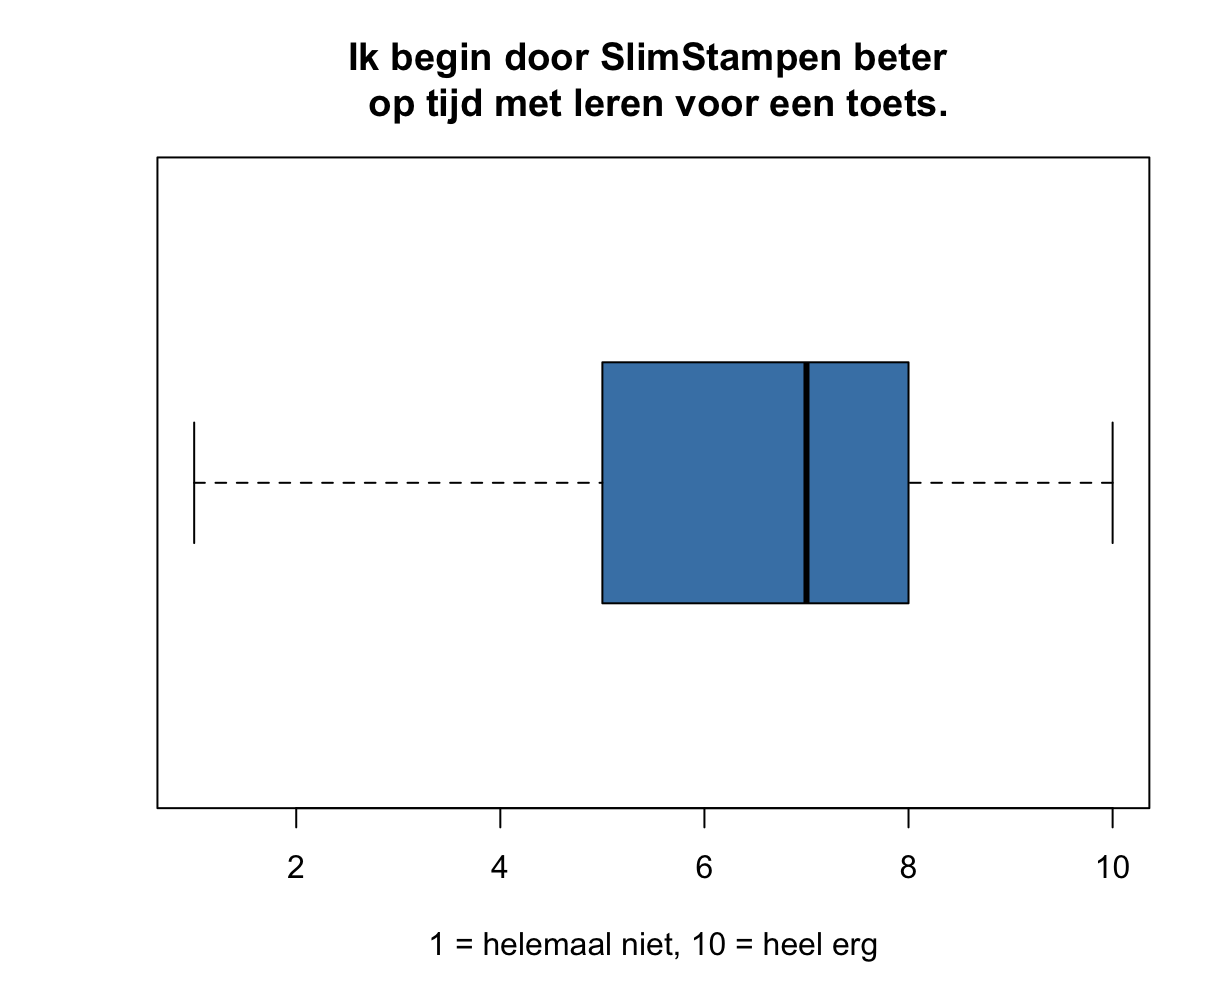
\includegraphics[width=65mm]{images/29-OpTijdBeginnenLeren.png} &   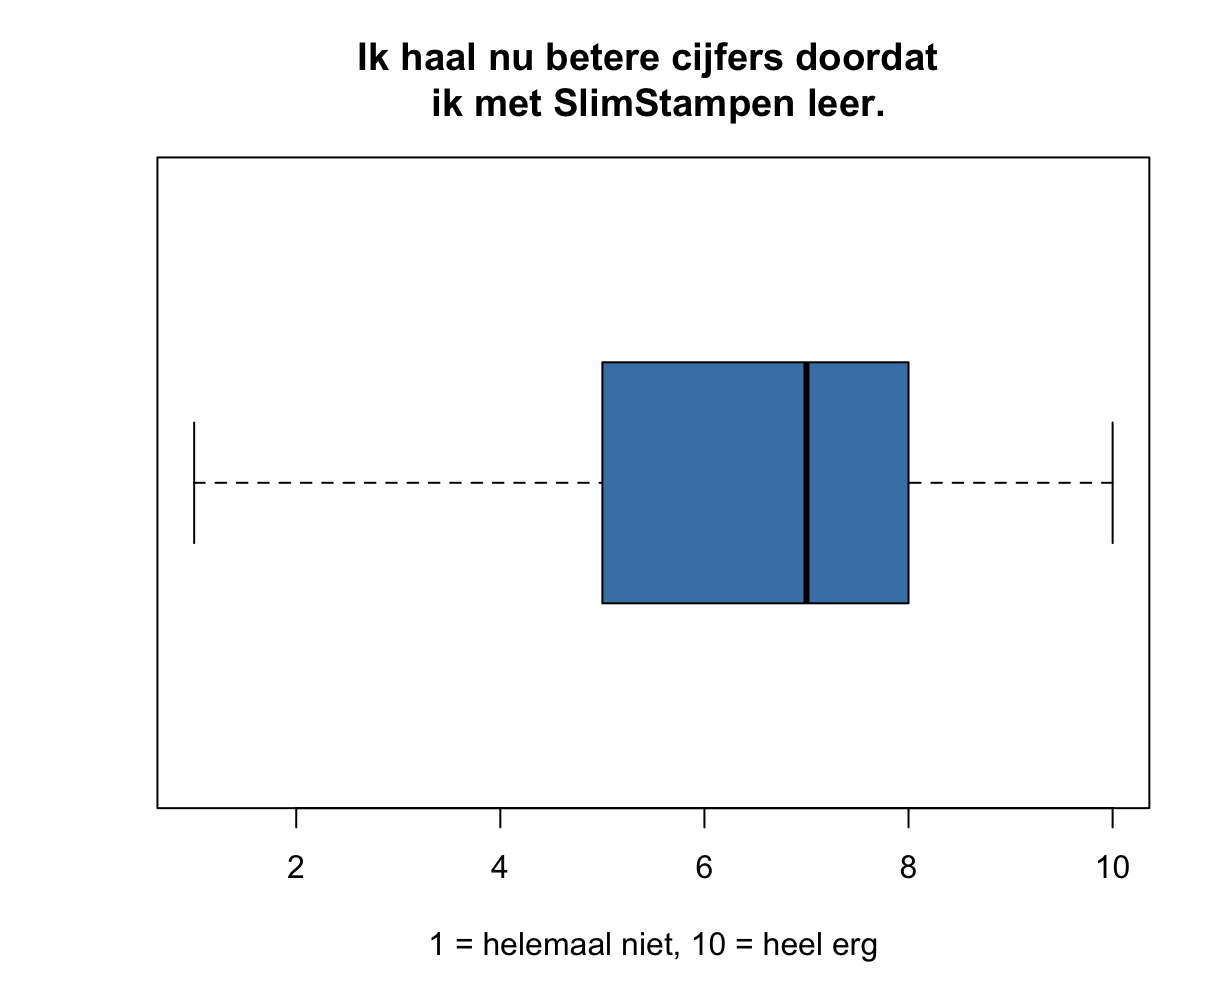
\includegraphics[width=65mm]{images/30-BetereCijfers.png} \\
        (c) $\overline{X}$ = 6.192, N=281, NA = 56  & (d) $\overline{X}$ = 6.529, N=280, NA = 57  \\[6pt]
        \end{tabular}
        \caption{indicatoren voor hogere motivatie}
        \label{fig:motivatie2}
        \end{figure}

Leerlingen die het gevoel hebben competent te zijn, zijn over het algemeen gemotiveerder voor school. Op de vraag of de leerlingen zich 
zekerder voelen op school over hun competentie door het gebruik van SlimStampen zijn leerlingen over het algemeen best positief 
(zie figuur \ref*{fig:motivatie2}(a)). Op de vraag of ze het fijn vinden dat ze door het gebruik meer hun eigen tijd kunnen indelen in plaats van dat de docent het toetsmoment bepaalt zijn verreweg de meeste leerlingen positief. Hier spreken we de leerlingen aan op hun autonomie. Je ziet in figuur \ref*{fig:motivatie2}(b) dat hier maar een paar leerlingen negatief op beantwoorden. Een paar outliers van leerlingen die zelfs ronduit negatief zijn. Dit zouden leerlingen kunnen zijn die ''zomaar'' iets hebben ingevuld, maar dat idee heb ik niet. Daar kom ik nog op terug in paragraaf 6.6. Als we naar de zelfdeterminatietheorie kijken van Deci en Ryan dan is het belangrijk dat leerlingen autonomie en competentie ervaren. Dit zijn twee van de drie basisbehoeften van de leerling. Deze worden door het gebruik van SlimStampen aangesproken.

De vraag ''Ik begin door SlimStampen beter op tijd te leren voor een toets'' van figuur \ref*{fig:motivatie2}(c) lijkt erg op de vraag van figuur \ref*{fig:motivatie}(d). Ik heb deze vraag wat meer toegespitst op specifiek het leren van een toets. Hier beantwoorden leerlingen over het algemeen ook iets positiever op dan de algemenere vraag over het eerder beginnen. Opvallend is dat de verdeling van de volgende vraag over het behalen van hogere cijfers met SlimStampen erg lijkt op het eerder beginnen met het leren van de toets. Het gemiddelde is zelfs iets hoger zoals je ziet in figuur \ref*{fig:motivatie2}(d).

Als conclusie kan ik stellen dat SlimStampen een positieve invloed heeft op de motivatie van de leerling. Leerlingen voelen zich zekerder over hun kunnen, vinden het fijn dat ze meer autonomie hebben en beginnen eerder met leren voor een toets. Dit alles leidt tot betere cijfers.

\subsection{Leerstrategieën}
\begin{figure}
    \begin{tabular}{cc}
      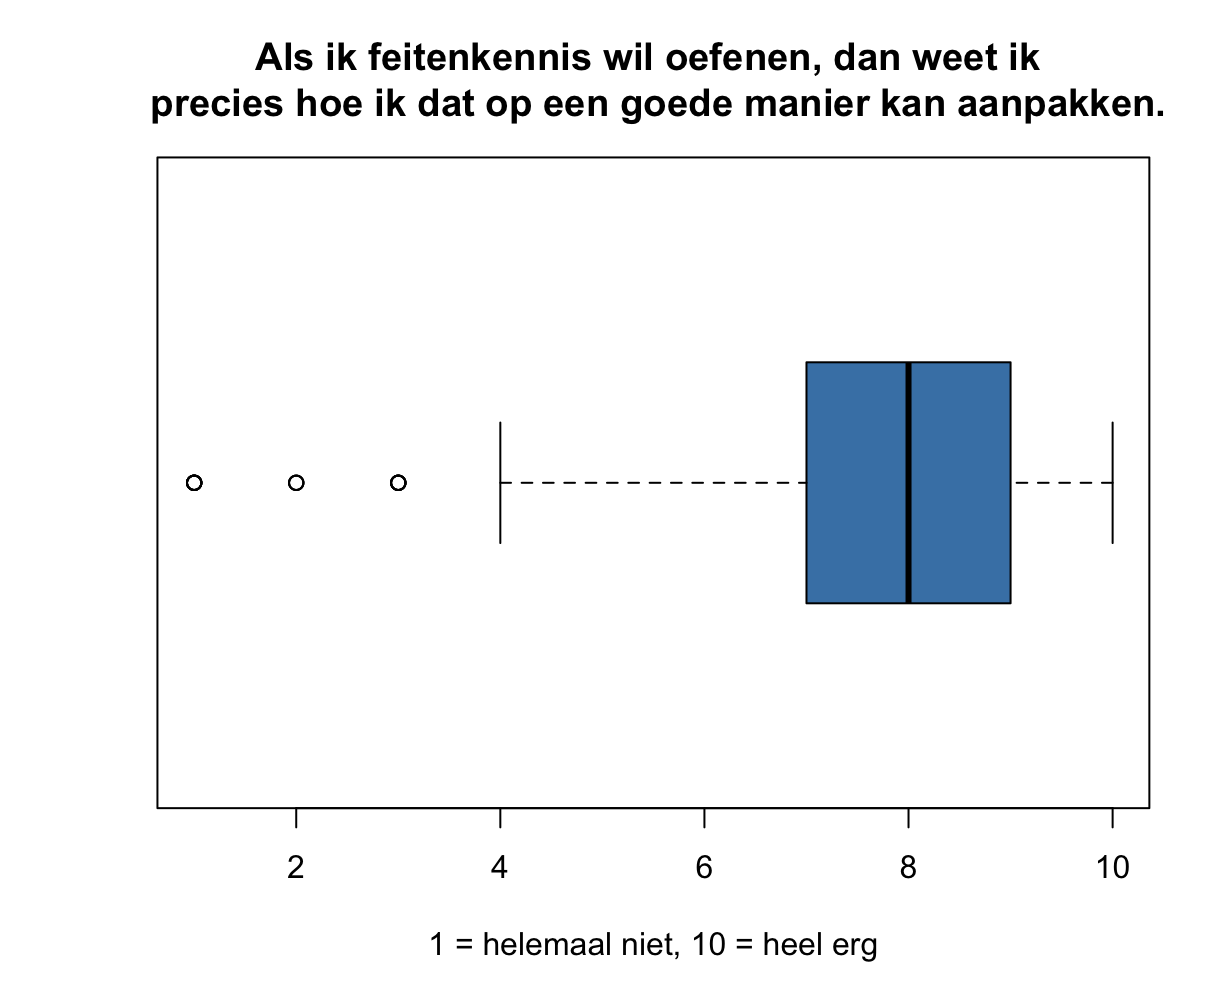
\includegraphics[width=65mm]{04-WeetAanpakken.png} &   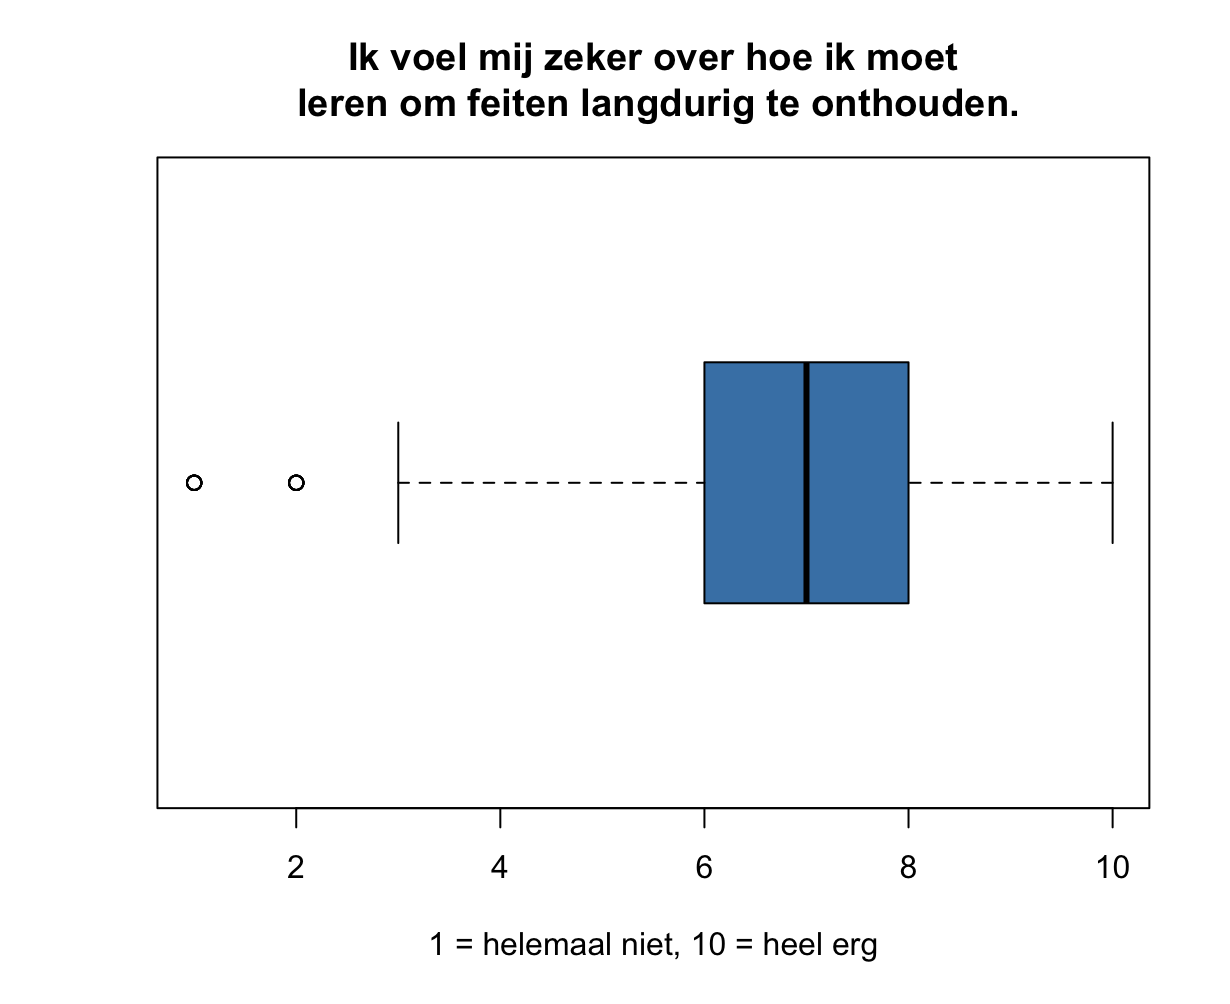
\includegraphics[width=65mm]{06-zekerOverOnthouden.png} \\
    (a)  $\overline{X}$ = 7.634, N=333, NA = 4 & (b) $\overline{X}$ =  6.83, N=335, NA = 2 \\[6pt]
    \multicolumn{2}{c}{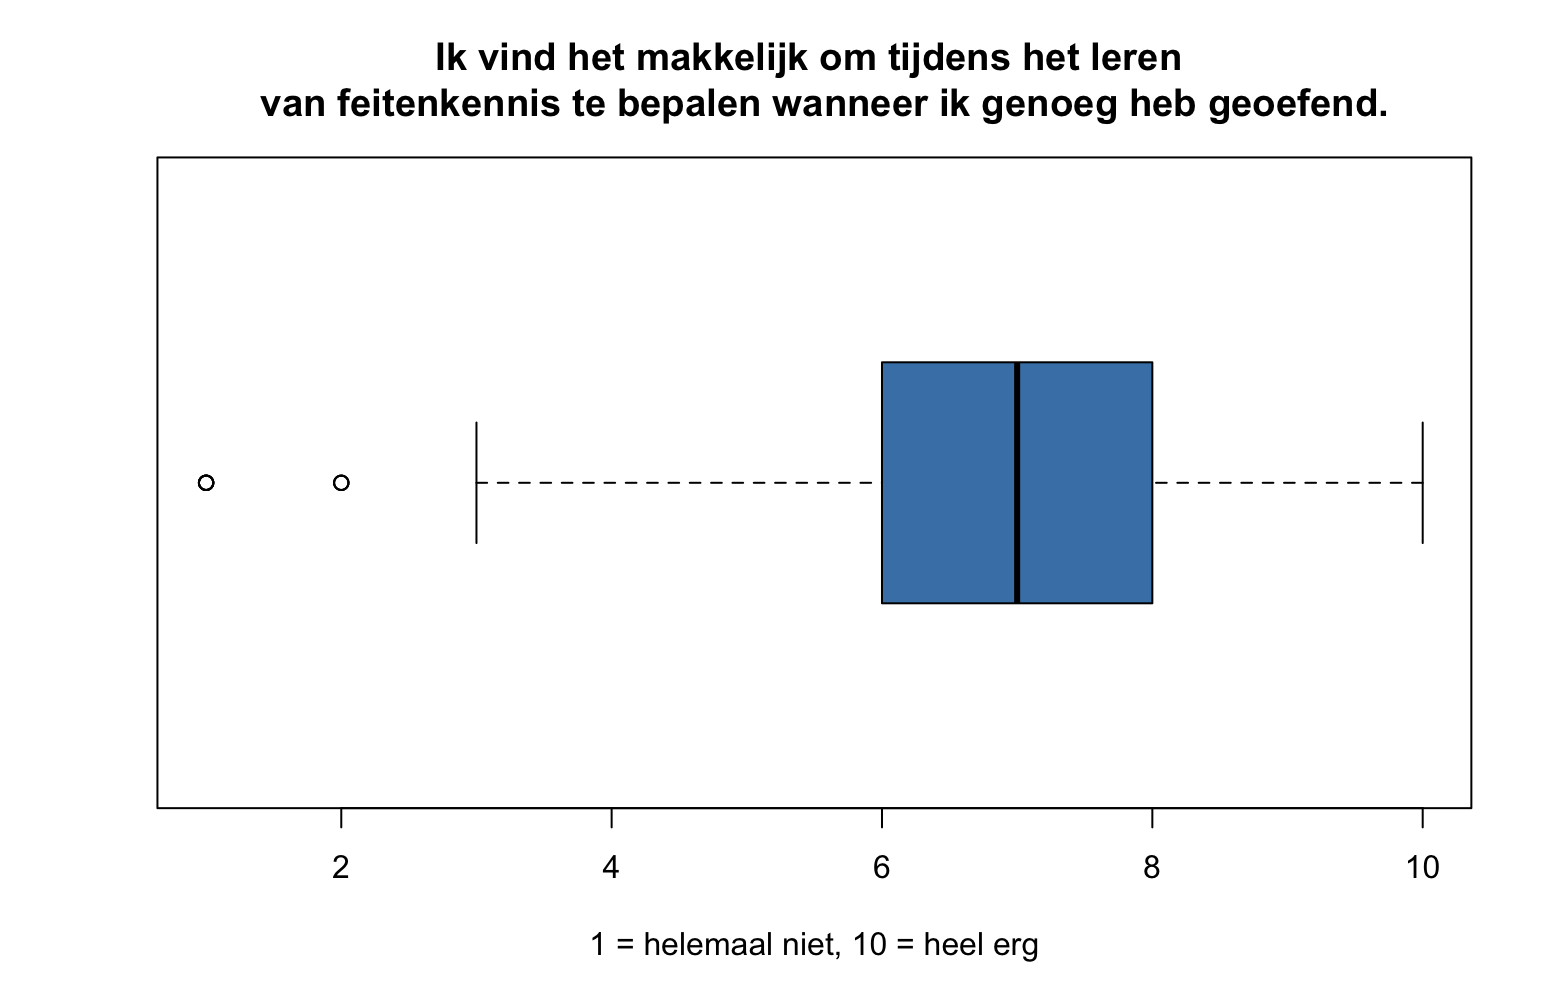
\includegraphics[width=65mm]{05-bepalenGenoegGeoefend.png} }\\
    \multicolumn{2}{c}{(e) $\overline{X}$ = 7.224, N=331, NA = 6}
    \end{tabular}
    \caption{kennis over leerstrategieën}
    \label{fig:leerstrategie}
    \end{figure}

    \begin{figure}
        \begin{tabular}{cc}
          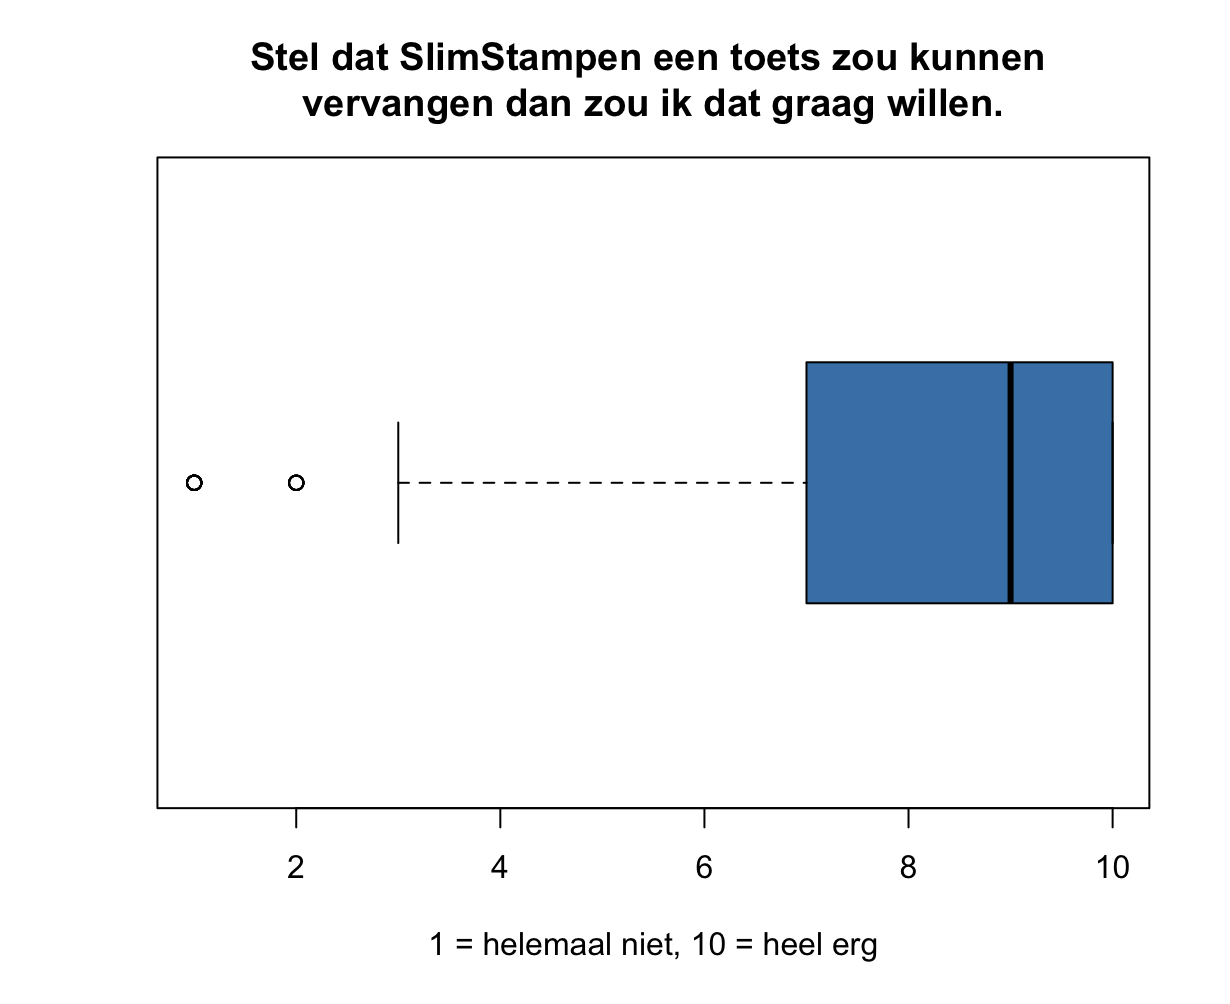
\includegraphics[width=65mm]{25-ToetsVervangen.png} &   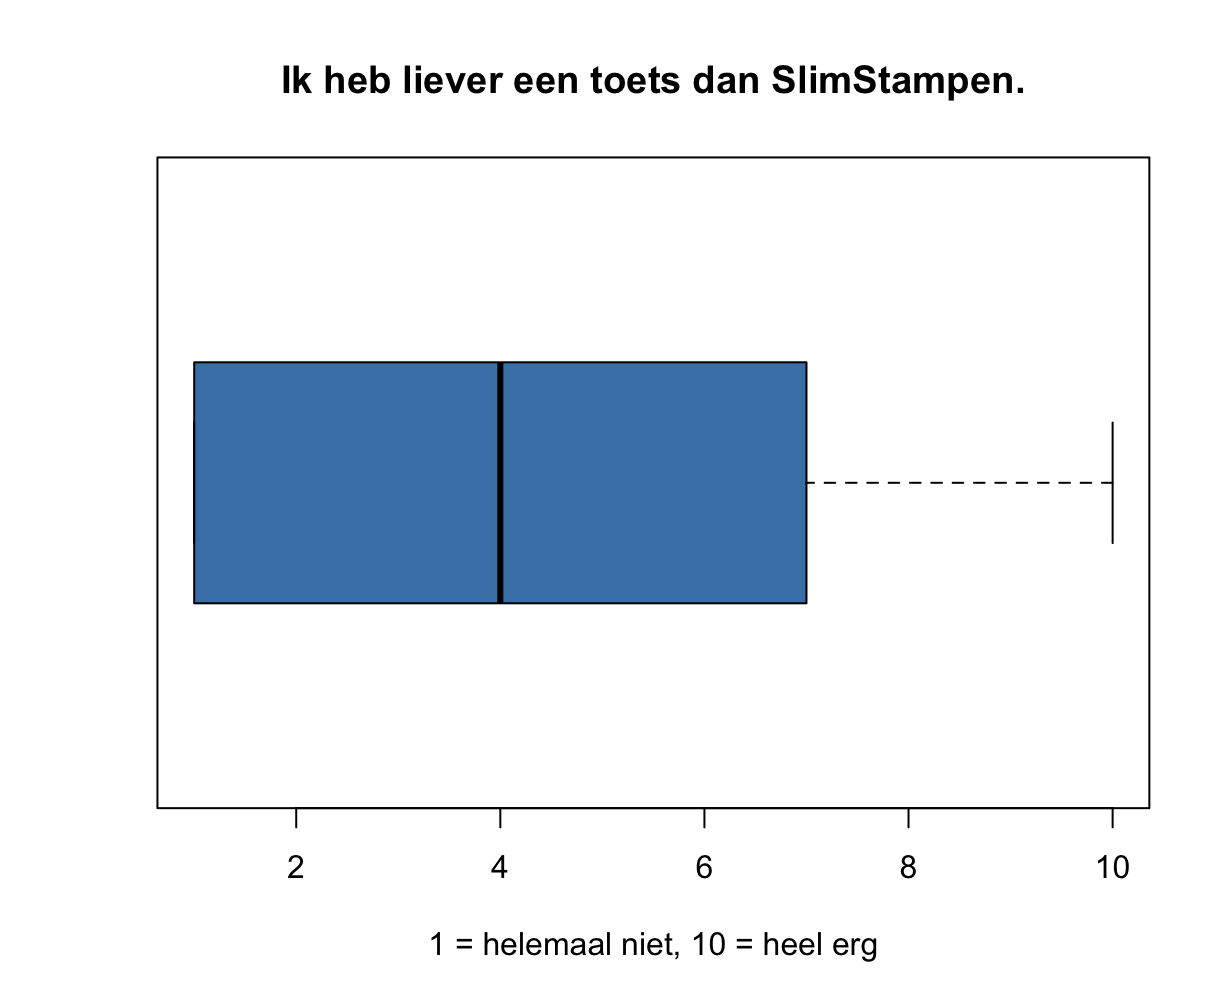
\includegraphics[width=65mm]{26-LieverToets.png} \\
        (a)  $\overline{X}$ = 7.841, N=283, NA = 54 & (b) $\overline{X}$ =  4.461, N=284, NA = 53 \\[6pt]
        \end{tabular}
        \caption{Evaluatie: toetsen of SlimStampen}
        \label{fig:evaluatie}
        \end{figure}

De eerste vragen van de enquête gingen over de kennis van de leerling over leerstrategieën. Er waren drie vragen waarbij de respondenten op een schaal van 1 tot 10 konden aangeven hoe erg ze het met de stelling eens waren. Deze drie vragen laten zien dat leerlingen over het algemeen best zeker zijn over hun kennis van leerstrategieën. Zoals je in de drie boxplots kan zien in figuur \ref*{fig:leerstrategie}. 

\begin{center}
    \begin{tabular}{|c|c|} 
    \hline
         keuzemogelijkheid & frequentie (N=337) \\
     \hline
     Op verschillende dagen de stof herhalen & 189 \\ 
     Mezelf laten overhoren door familie of vrienden & 170  \\ 
     Een overhoorprogramma op mijn computer of mobiel & 163 \\
     De feiten herhaald hardop lezen of overschrijven & 144  \\ 
     Andere & 36 \\
     \hline
    \end{tabular}
    \end{center}

De meerkeuze vraag ''Om feitenkennis te onthouden gebruik ik deze strategieën?'' laat zien dat leerlingen meerdere strategieën hanteren. Zij konden ook een eigen strategie invullen en daar waren deze verschillende antwoorden:
\emph{
'een briefje op plekke hangen waar ik vaak kom bijv. wc en dan herhalen als ik daar ben', 'ik schrijf de betekenissen van de feiten ergens op', 'Samenvattingen maken', 'slimstampen', 'videos', 'chatGPT die het overhoord', 'muziek luisteren en het meerdere keren doornemen', 'Gewoon normaal' en 'ezels bruggetjes'.}
SlimStampen werd meerdere keren apart genoemd, terwijl dit gebruik binnen een antwoord had gepast (namelijk, Een overhoorprogramma gebruiken). Meer dan de helft van de leerlingen gebruikt meerdere strategieën, waarbij herhalen en laten overhoren het meest gebruikt worden. Veel leerlingen zijn zich bewust van de voordelen van het spacing effect en retrieval practice.

Mijn conclusie is dat leerlingen over het algemeen goed denken te weten hoe ze feiten moeten leren en onthouden. Ze gebruiken meerdere strategieën en zijn zich bewust van het belang van het spacing effect en retrieval practice. SlimStampen past goed in deze strategieën. Het is een overhoorprogramma dat de leerling zelfstandig kan gebruiken en dat rekening houdt met het spacing effect.

\subsection[Evaluatie]{Evaluatie van SlimStampen}
Bij de evaluatie van SlimStampen was er sprake van twee gesloten vragen met schaal van 1 tot en met 10 en twee open vragen. De vragen gingen allemaal over het oordeel van de repondenten over het gebruik van SlimStampen. De gesloten vragen zijn tegengesteld gevraagd ter controle.
In figuur \ref*{fig:evaluatie}(a) en (b) valt te concluderen dat veel leerlingen graag zien dat SlimStampen toetsen vervangt. De controlevraag in (b) laat een iets minder negatieve score zien op de vraag of ze liever een toets hebben dan dat (a) een positieve score heeft. De spreiding van de antwoorden ligt bij (b) ook hoger dan bij (a). Dat kan liggen aan het feit dat alle andere vragen uit de enquête positief gesteld zijn. Als ze even niet opletten kunnen de repondenten het verkeerde antwoord hebben gegeven.

    \begin{center}
        \begin{tabular}{|c|c|}
        \hline
             Bij welke vakken SlimStampen & frequentie (N=337) \\
         \hline
         Frans & 217 \\ 
         Duits & 152  \\ 
         aardrijkskunde & 129 \\
         Engels & 86  \\ 
         geschiedenis & 21 \\
         biologie & 9 \\
         wiskunde & 2 \\
         andere & 8 \\
         \hline
        \end{tabular}
        \end{center}
Je ziet dat de leerlingen van het Metis Montessori Lyceum al bij heel veel vakken SlimStampen gebruiken. Er worden ook vakken genoemd waarvan ik niet wist dat ze daar ook met SlimStampen leren. Bij de categorie 'andere' werden genoemd: 'Grieks' en 'natuurkunde' 'scheikunde'. Dit zijn vakken waar wij op ons SlimStampen domein geen lessen hebben staan. Het kan heel goed dat de leerlingen op het algemene domein app.slimstampen.nl de lessen oefenen voor deze vakken.

\begin{center}
    \begin{tabular}{|c|c|} 
    \hline
         Waarom gebruik je SlimStampen & frequentie (N=283) \\
     \hline
        verplicht/moet & 47 \\
        je krijgt punten op de toets & 18 \\
        handig/helpt & 128 \\
        neutraal & 63 \\
        nietszeggend, niet serieus & 27 \\
     \hline
    \end{tabular}
    \end{center}

De vraag ''Waarom gebruik je SlimStampen?'' was een open vraag. De leerlingen werden geheel niet gestuurd in hun antwoorden. Dat heeft voor een deel nietszeggende of neutrale antwoorden opgeleverd. Na de verschillende antwoorden bestudeerd te hebben, heb ik de antwoorden ingedeeld in verschillende categorieën. Er wordt met het programma gewerkt vanuit een negatieve keuze (het moet) en een positieve keuze (handig of helpt). Er zijn leerlingen (47) die duidelijk SlimStampen doen vanuit een verplichting. Verder zijn er ook leerlingen (18) die aangeven dat ze het doen vanuit een stimulans, ze kunnen extra punten verdienen voor de toets door te laten zien dat ze hebben geoefend met SlimStampen. Ook geeft een aantal leerlingen neutrale antwoorden, waar geen positieve of negatieve keuze in zit, zoals bijvoorbeeld 'om te leren' of 'voor Frans'. Ook werd een aantal antwoorden gegeven die duidelijk niet serieus waren. Uit de gegeven antwoorden blijkt dat de meeste leerlingen SlimStampen gebruiken uit een positieve keuze. 'Het is handig', 'Het helpt bij leren' en 'Omdat ik het een keer had uitgeprobeerd (daar kregen we extra punten voor bij Frans) en ik had de woordjes heel goed onthouden, dus nu gebruik ik het vaker'. Het laatste antwoord geeft aan dat de stimulans heeft geholpen om de ervaring op te doen. De leerling heeft vervolgens een zelfstandige positieve keuze gemaakt om het vaker te gebruiken.

Ik kan concluderen dat leerlingen SlimStampen vooral gebruiken omdat ze het handig vinden en het helpt bij het leren. Er zijn ook leerlingen die het doen omdat het moet, maar dat is een minderheid. De stimulans van punten verdienen voor de toets motiveert leerlingen om het te gebruiken. Het vervangen van toetsen door SlimStampen wordt door de meeste leerlingen positief ontvangen.

\subsection{Onverwachte onregelmatigheid}
Na het afnemen van de enquête kwam een onregelmatigheid bij het gebruik met SlimStampen in de vierde klas naar boven. Uit de leerdata bleek dat een aantal leerlingen veel te snel ''kroontjes'' haalde. Bij het bestuderen van de leerdata zag ik dat leerlingen voor ieder antwoord dat ze gaven een reactietijd van exact 500 milliseconden hadden. Deze tijd is vrijwel niet mogelijk voor een mens en het is zeker uitgesloten dat een mens bij ieder antwoord exact deze tijd zou halen. Het vermoeden was dat een computer had beantwoord, met andere woorden hier was sprake van ''een bot''. 

De leerlingen die deze bot hadden gemaakt waren zo gevonden, de code stond op github, een site waar programmeurs hun code delen en samenwerken. Met een script ontdekten we dat 43 leerlingen de bot hadden gebruikt om kroontjes te halen. Het aantal behaalde kroontjes zou omgezet worden in een cijfer en een toets vervangen. Daarmee was dit een serieus probleem. Waarom hadden deze leerlingen hiervoor gekozen?

Hiermee kreeg ik een mogelijkheid tot onverwachte en extra informatie voor mijn onderzoek. Onder de leerlingen die de bot hadden gebruikt heb ik een vragenlijst gestuurd om te ontdekken wat hun beweegredenen waren om de bot te gebruiken. Twaalf leerlingen hebben de moeite genomen om de vragen uitgebreid te beantwoorden, dat is 27,9 procent van de bot gebruikers. Dit betekent dat deze informatie misschien niet heel representatief is, maar omdat het inhoudelijk interessant en relevante informatie is, heb ik het besloten om dit toch in dit onderzoek mee te nemen. 

In de antwoorden op de vraag waarom ze de bot hebben gebruikt (die je kan lezen in Bijlage A) zie je dat de leerlingen over het algemeen niet direct tegen SlimStampen zijn, maar meer tegen de manier waarop het is ingezet. Dit is waardevolle feedback. Uit de andere antwoorden (de vragen staan ook in bijlage A) lees ik dat de leerlingen begrijpen waarom SlimStampen werkt. Zij geven wat meer flexibiliteit als verbeterpunt. Acht van deze leerlingen willen liever een toets dan SlimStampen, maar vier hebben toch liever SlimStampen dan een toets. Een leerling geeft aan de werking van SlimStampen te begrijpen, maar denkt dat je met een woordenlijst ernaast vals kan spelen door af te kijken. Dit is niet helemaal waar, want dat levert een te lange reactietijd op. De leerling begrijpt SlimStampen dus niet helemaal. Ik ben het niet altijd helemaal met deze leerlingen eens, maar ze hebben goede punten en we maken het onderwijs samen. Docenten en leerlingen. Hier kunnen en moeten we wat mee. Daar kom ik bij de conclusie en aanbevelingen op terug.
\newpage
\section{Conclusie, reflectie en aanbevelingen}
Het doel van dit onderzoek was om, op grond van een literatuurstudie en een enquête onder leerlingen, inzicht te geven in de waarde van SlimStampen op een middelbare montessorischool. Ik heb de waarde vertaald naar een viertal belangrijke kenmerken van het montessorionderwijs: de voorbereide omgeving, normalisatie, motivatie en leerstrategieën. Daarnaast heb ik door middel van een enquête onder leerlingen het gebruik van SlimStampen geëvalueerd.

De voorbereide omgeving is een belangrijk kenmerk van het montessorionderwijs. SlimStampen is een digitale leeromgeving die de leerling helpt bij het leren van feitenkennis. Uit de enquête blijkt dat leerlingen positief zijn over de duidelijkheid en overzichtelijkheid van SlimStampen. Ze weten wat ze moeten doen en kunnen er zelfstandig mee aan de slag. Dit past goed bij het idee van de voorbereide omgeving van Maria Montessori.

De normalisatie van de leerling is een ander belangrijk kenmerk van het montessorionderwijs. Normalisatie raakt de taakaanvaarding van de leerling. Uit de enquête blijkt dat SlimStampen helpt bij de concentratie en dat leerlingen gefocust aan het werk gaan. Ze laten zich niet snel afleiden en voelen zich zekerder over hun kunnen. Dit past goed bij wat Maria Montessori zag als normalisatie.

De motivatie van de leerling is een derde belangrijk kenmerk van het montessorionderwijs. Uit de enquête blijkt dat SlimStampen een positieve invloed heeft op de motivatie van de leerling. Leerlingen vinden het fijn dat ze meer autonomie hebben en beginnen eerder met leren voor een toets. Dit alles leidt tot betere cijfers.

Leerstrategieën zijn een vierde belangrijk kenmerk van het montessorionderwijs. Uit de enquête blijkt dat leerlingen over het algemeen goed denken te weten hoe ze feitenkennis moeten leren en onthouden. Ze gebruiken meerdere strategieën en zijn zich bewust van het belang van het spacing effect en retrieval practice. SlimStampen past goed in deze strategieën. Het is een overhoorprogramma dat de leerling zelfstandig kan gebruiken en dat rekening houdt met het spacing effect.

De evaluatie van SlimStampen bij de leerlingen laat zien dat zij over het algemeen positief zijn over het gebruik van SlimStampen. Zij vinden het handig en het helpt bij het leren. De meeste leerlingen zien graag dat SlimStampen toetsen vervangt. Dit past goed bij het idee van het zelfstandig werken en de vrije keuze in het montessorionderwijs.

Het antwoord op de onderzoeksvraag is dat SlimStampen een waardevolle aanvulling is op het montessorionderwijs. Het draagt bij aan de voorbereide omgeving, normalisatie, motivatie en leerstrategieën van de leerling. Het is een digitale leeromgeving die de leerling helpt bij het leren van feitenkennis en die goed aansluit bij de principes van het montessorionderwijs. Daarmee draagt dit onderzoek bij aan de verdere ontwikkeling van het montessorionderwijs en kan ik met dit onderzoek onderbouwen dat SlimStampen een waardevolle aanvulling is op het montessorionderwijs in het gesprek met mijn collega's, de schoolleiding en de ontwikkelaars van SlimStampen.

Tijdens mijn literatuurstudie heb ik mij verdiept in de betekenis en belang van normalisatie. Daarbij ben ik teruggegaan naar het gedachtegoed van een aantal verlichtingsfilosofen. Ik ontdekte veel ideeën van het montessorionderwijs in deze filosofen. Maria Montessori had hier mijns inziens meer krediet kunnen geven aan hen. Ik vond de zoektocht naar de achtergrond van haar ideeën waardevol. Het heeft mij meer diepgang en vertrouwen gegeven in mijn rol als docent. Ik vind de ontbrekende verwijzingen in de boeken van Maria Montessori een gemis. Wellicht is een verklaring dat ze zichzelf een wetenschapper vond en geen filosoof. Ze manifesteerde zichzelf als empirist door de nadruk te leggen op het observeren en minder als rationalist, terwijl ze mijns inziens wel degelijk ook rationalist was.

Een belangrijke bevinding voor mij is dat drie kenmerken die ik beschreven heb in belangrijke mate samenhang vertonen. De voorbereide omgeving is van belang voor een normalisatie en uit de normalisatie vloeit motivatie. Dit past weer bij het idee van Maria Montessori over kosmisch onderwijs. Alles hangt met elkaar samen.

De spanning tussen vrijheid en discipline in het onderwijs vind ik een fascinerend gegeven. Dat was voor mij een aandachtspunt tijdens dit onderzoek. Ik begrijp nu veel beter wat met deze begrippen, in relatie met Maria Montessori's \emph{vrijheid in gebondenheid}, wordt bedoeld. Voor veel buitenstaanders staat montessorionderwijs voor vrijheid. Dit is een sterke misvatting. Discipline is een belangrijk element binnen het montessorionderwijs. Niet de opgelegde (autoritaire) discipline, maar een zelfgekozen discipline. Alleen met een zelfgekozen discipline kan je werkelijke vrijheid ervaren, omdat in een samenleving altijd regels zijn waar je je aan moet houden. Deze regels kunnen je een gevoel van beperking geven als je deze niet aanvaard. Dus alleen als je deze regels accepteert kan je je vrij voelen. De ene leerling reageert verontwaardigd bij een toets of een schoolregel, de andere leerling voelt zich vrij in zijn of haar keuzes. De zelfgekozen diepe concentratie wanneer je werkt, het werken zonder dat de docent zegt dat je aan het werk moet. Dat is de discipline of normalisatie waar Maria Montessori naar op zoek is bij de leerling. Uit deze normalisering volgt veelal een hogere motivatie voor school.  

Uit de data uit de enquête blijkt dat leerlingen positief zijn over SlimStampen als montessorimateriaal. Het zelf indelen van de tijd, de helderheid van het materiaal en het eventueel vervangen van toetsen door SlimStampen wordt erg gewaardeerd. Ik zelf zie SlimStampen ook als leermiddel voor het aanleren van leerstrategieën, zoals herhalen en ophalen, dit wordt niet door alle leerlingen gezien, maar veel leerlingen zien wel deze waarde van SlimStampen. Veel leerlingen zijn al bekend met deze leerstrategieën. Leerlingen geven aan goed in een concentratie te komen bij het gebruik van SlimStampen. Zij laten zich niet snel afleiden als ze met deze taak bezig zijn. Het werken met SlimStampen geeft de leerlingen de mogelijkheid om wat meer autonomie te ervaren.

SlimStampen helpt bij de motivatie voor leerlingen, dat blijkt uit het feit dat ze het leren met SlimStampen leuker vinden dan zelf rijtjes te moeten leren. Het leren met SlimStampen geeft een positief gevoel achteraf. De leerlingen vinden het fijn om meer hun eigen tijd in te delen. Ze voelen zich zekerder over hun kunnen op school door SlimStampen en hebben het idee dat ze nu hogere cijfers halen. SlimStampen zorgt voor een gevoel van competentie bij veel leerlingen.

Bij de vakken Frans, Duits, aardrijkskunde en Engels wordt SlimStampen bij ons op school al veelvuldig ingezet. Leerlingen zien uit naar de mogelijkheid dat SlimStampen een toets kan vervangen. Vijfenzeventig procent van de leerlingen staat hier positief tot zeer positief tegenover. Een klein aantal leerlingen niet. En daar moeten we meer onderzoek naar doen.

Bij het vak Engels in de vierde klas werd een toets dit jaar daadwerkelijk vervangen door SlimStampen. Je zou denken gezien de resultaten van mijn onderzoek dat dit toegejuicht zou worden. Dit is niet het geval bij een aantal leerlingen. Het vervangen van de toets met dit leeralgoritme heeft een aantal leerlingen ertoe gezet om een bot te ontwikkelen en te gebruiken. De computer behaalde de vereiste kroontjes in plaats van de leerlingen. Waar kwam dit gedrag vandaan? Hier heb ik de leerlingen die de bot hebben gebruikt naar gevraagd. De resultaten waren verhelderend. Van de leerlingen die de bot hebben gebruikt staan de meesten niet negatief tegenover SlimStampen, maar tegenover de manier waarop dit is ingezet. 

Dit is waardevolle informatie die ik ook heb gedeeld met Universiteit Utrecht, want dit vraagt om meer onderzoek. Ik dacht dat we de leerlingen meer autonomie gaven door niet een toets te geven op een door ons vastgestelde datum. Dit werd niet zo ervaren. De leerlingen voelden zich door ons gedwongen om alle woorden te leren. Ze geven aan dat ze al Engels kunnen en de toets gewoon zouden maken. Hier zouden ze zonder al te veel te leren al een voldoende voor halen. Bij SlimStampen haal je pas een kroontje als je 100 procent van de woorden kent. Dat vergt een hele andere benadering. De docenten moeten goed nadenken over welke woorden ze echt vinden dat de leerlingen moeten weten. Welk percentage is voldoende? Dit is een belangrijk punt van aandacht.

We moeten ook niet vergeten dat de leerlingen die de bot hebben gebruikt een kleine groep is. De meeste leerlingen hebben SlimStampen gewoon gebruikt zoals het bedoeld is en zoals de docenten het bedoeld hadden. Dan kom je tot een belangrijke vraag: kunnen we alle leerlingen tegemoet komen in al hun wensen? Het feit dat de leerlingen die de bot hebben gebruikt vaak aangeven dat het bij Duits wel juist is gebruikt en bij Engels niet, geeft aan dat er een verschil is in de manier waarop SlimStampen wordt ingezet. Dit is een volgend belangrijk punt van aandacht.

Ik heb in dit onderzoek een aantal aanbevelingen gedaan voor de school en de ontwikkelaars van SlimStampen. Ik denk dat het belangrijk is dat de school goed nadenkt over de manier waarop SlimStampen wordt ingezet. Aandachtpunten hierbij zijn:
\begin{itemize}
    \item Hoeveel procent van de feiten moet een leerling beheersen om voldoende kennis te hebben volgens de docenten?
    \item Hoe zetten we SlimStampen in, moet het een toets vervangen of is het een hulpmiddel voor de leerling?
    \item Alle docenten op de hoogte stellen van mijn bevindingen en samen met hen kijken naar de manier waarop SlimStampen wordt ingezet.
    \item Wat is essentiele feitelijke kennis en wat is extra kennis? Alleen de essentiele kennis moet in SlimStampen.
\end{itemize}

Ik heb inmiddels binnen het hele MSA de rol van coördinator SlimStampen. Docenten van de diverse scholen weten mij steeds beter te vinden en vragen nu al naar resultaten van mijn onderzoek. In dit onderzoek heb ik mij vooral gericht op de leerlingen. Ik denk dat het belangrijk is om ook de docenten te betrekken bij de evaluatie van SlimStampen. Zij kunnen waardevolle feedback geven over de inzet van SlimStampen in de klas. Ik denk dat het goed is om een werkgroep op te richten met docenten die SlimStampen inzetten in de klas. Zij kunnen samen met mij kijken naar de resultaten van de enquête en de aanbevelingen die ik heb gedaan. Zo kunnen we samen werken aan een betere inzet van SlimStampen in de klas. 

Met MemoryLab en Universiteit Utrecht heeft het MSA nog voor twee jaar subsidie om verder onderzoek te doen naar het gebruik van een leeralgoritme in het middelbaar onderwijs. Een aantal van bovenstaande aandachtpunten zal daarin aan bod komen. Ik hoop hier nog een belangrijke rol in te kunnen vervullen.
\newpage
\appendix
\section{Bijlage}
\emph{Waarom heb je besloten de bot te gebruiken?}

\begin{enumerate}
    \item De Engels woordenlijst van slimstampen duurde erg lang om te maken en het voelde meer als een rot klusje dan iets waar ik van leerde. Ik besloot om de bot te gebruiken om mezelf de tijd en moeite te besparen voor iets wat mij onnodig leek.
    \item Ten eerste wil ik zeggen dat ik de bot alleen voor Engels heb gebruikt, niet voor Duits want bij Duits werkt het goed. je leert woordjes en die woordjes komen samen met grammatica in de toets. Bij Engels daarentegen is SlimStampen een apart cijfer wat ik raar vind.
    \item ik wou het uittesten onze klas hoefte volgends mij geeneens slim stampen woordjes te maken
    \item te veel opdrachten voor engels
    \item Het was te repetitief, herhaalde zichzelf te vaak. Vaker dan hoort.
    \item ik heb de bot puur en alleen gebruikt voor engels, waar je 12 woordenlijsten nederlands-engels en engels-nederlands moet 'leren' om geen 1 op je eind raport te krijgen. het enige nadeel is dat deze lijsten niet altijd correct zijn vertaald waardoor het vaak moeilijk is de lijsten te maken, zelfs al ken ik alle woorden goed en kan ik ze juist in een zin verwerken.
    \item Ik vind Slimstampen oprecht een goed systeem. De reden waarom ik de bot heb gebruikt is omdat Engels heel veel was. Bij sommige vakken is het goed uitgevoerd zoals bij Duits en bij sommige vakken is het heel slecht uitgevoerd zoals bij Engels. Bij Duits zijn de lijsten van slimstampen facultatief, maar je krijgt wel bonus punten als je ze maakt. Ik vind dit een win win situatie, want als je goed bent in Duits hoef je dus niet de lijsten te doen en als je slecht bent in Duits dan zou ik de lijsten maken zodat je de woordjes beter leert en zodat je de bonuspunten kan krijgen. Bij Engels is het verplicht, hierdoor moeten de mensen die goed zijn in Engels nog steeds heel veel tijd erin stoppen, waardoor je uiteindelijk heel gedemotiveerd wordt. Wat Engels ook doet is in plaats van 12 lijsten geven voor de 12 units geeft het je 24 lijsten, 12 voor NL-ENG en 12 voor ENG-NL. Hierdoor doe je dubbel zoveel werk waardoor het uiteindelijk voelt alsof je oneindig lang bezig bent. Heel veel leerlingen vonden dit te veel werk. Dat is ook de reden dat [naam verwijdert ivm privacy - MM] en [naam verwijdert ivm privacy - MM] die bot hebben gemaakt. Ik denk dat het beter zou zijn als de Engels lijsten hetzelfde zou zijn als de Duits lijsten. Voor de rest vind ik slimstampen een geweldig alternatief voor grote woordenschattoetsen en een handige manier voor het stampen van woorden, met uitzonderingen voor hoe slecht de Engels lijsten zijn.
    \item 1. Omdat ik geen zin had om al die honderden woordjes Engels te ''leren''. Ik kende al die woorden van Engels al.\\
     2. Zelfs als ik de woorden niet zou kennen, vind ik het fijn om niet geforceerd voor een cijfer tweehonderd keer hetzelfde te moeten typen. Het voelt als breindood typen, vooral dus als je de woorden al kent. Ik zou het dus fijner vinden als de woordenlijsten (zoals bij Duits) als optioneel hulpmiddel voor woordjes bij toetsen zijn.\\
    3. Een programma schrijven met python en HTTP leek mij vele malen leuker dan dat getyp.\\   
    4. Het is sowieso nog beter om woordjes met zinnen te leren in plaats van de woordjes afzonderlijk te toetsen, dan weet je alsnog niet hoe het in een zin zou passen in een andere taal (als je die taal nog echt niet goed kent).''\\
    \item Ik weet de woorden al, ik spreek al jaren dagelijks Engels. Ik vind dat het voor mij een verspilling van tijd is.\\
    \item geen zin om voor engels 16-30 uur woordjes te stampen die ik al ken. \\
    \item Ik had het gebruikt voor engels want we kregen daar 24 lijsten in een keer en dat kost best veel tijd.\\
    \item Omdat slimstampen erg lang duurt, de lijsten zijn niet praktisch (woorden die ook kloppen worden niet goedgerekend) en het systeem is niet prettig om te gebruiken. Met een bot gaat het sneller terwijl ik nog wel kan leren.\\
\end{enumerate}

Andere vragen aan deze leerlingen:\\
\begin{enumerate}
    \item Ik heb liever een toets dan SlimStampen...
    \item Ik denk dat ik snap waarom SlimStampen werkt?
    \item Als ik deze uitleg lees, snap ik meer van SlimStampen\\
     https://www.memorylab.nl/wetenschap/ en word ik positiever over het gebruik van SlimStampen?
    \item Wat zou er bij SlimStampen moeten verbeteren, zodat ik het wel met plezier gebruik?
    \item Dit wil ik nog kwijt...
\end{enumerate}

\newpage
\bibliographystyle{apacite} 
\bibliography{bibliography}

\end{document}